\documentclass[12pt,a4paper]{article}
\usepackage[utf8]{inputenc}
\usepackage{graphicx}
\usepackage{geometry}
\usepackage{booktabs}
\usepackage{array}
\usepackage{tabularx}
\usepackage[table]{xcolor}
\usepackage{longtable}
\usepackage{tikz}
\usepackage{float}

\newcolumntype{P}[1]{>{\raggedright\arraybackslash}p{#1}}
\newcolumntype{Y}{>{\raggedright\arraybackslash}X}
\setlength{\emergencystretch}{2em}

\begin{document}

% --- TITLE PAGE ---
\begin{titlepage}
    \centering
    \IfFileExists{uniba_logo.png}{\includegraphics[width=0.3\textwidth]{uniba_logo.png}\par\vspace{1cm}}{\vspace*{3cm}}
    {\scshape\LARGE University of Bari Aldo Moro \par}
    {\scshape\Large Computer Science Department \par}
    \vspace{1.5cm}
    {\huge\bfseries Database Systems Project Work: StageUp Inc. \par}
    \vspace{2cm}
    {\Large Student: Signorile Giacomo \par}
    \vfill
    {\large A.Y. 2024/2025 \par}
\end{titlepage}

\section{Requirements Collection}
The company "StageUp Inc." manages the rental and installation of audiovisual equipment for events through a decentralized operational structure. The organization consists of a central office and several operational depots distributed globally. Each depot is responsible for a specific geographical region, which is further subdivided into one or more municipalities. While the central office handles the coordination of bookings and administrative tasks, it does not manage physical setups; these are exclusively handled by the depots. Both the central office and the depots are characterized by a name, address, city/province, and the number of employees.
Customers, who can be classified as either individuals or companies, are identified by a unique alphanumeric code and their personal details. Services are requested through various channels, including phone, postal mail, email, or the corporate website. Bookings are categorized into several types, such as one-time requests, recurring services, seasonal contracts, or promotional rentals. Every booking is performed at a specific event location associated with a customer. Each location is defined by its address, house number, postal code, city, and province. Within a customer’s profile, each location is identified by a unique code and includes specific technical data, such as a setup time estimate and total equipment capacity.
Each operational depot manages one or more setup teams, which are limited by a maximum number of members. A team is identified by an identification code, a name, and the total number of installations performed. Teams are composed of members, for whom the system maintains personal data. Each booking record is comprehensive, storing the service type, date, duration, total cost, the specific team that handled the installation, and the detailed information of the customer who placed the order.

\section{Requirements Analysis}

\subsection{Choosing the correct level of abstraction}

\begin{itemize}
    \item \textbf{At line 3}, the address for the central office and depots is a little bit general, including also other information related to it such as city and province. Therefore, for address we assume that it represents street name, house number, zip code, city, and province.
    
    \item \textbf{At line 5}, the booking placement methods (phone, postal mail, email, website) are listed as channels. Therefore, we assume that "placement mode" is an attribute that handles one of the following values: \{Phone, Mail, Email, Website\}.
    
    \item \textbf{At line 8}, the setup time estimate and equipment capacity are general. We assume that the setup time is represented as a numeric value in minutes, while equipment capacity represents the maximum number of physical units the location can accommodate.
    
    \item \textbf{At line 10}, the "personal data" of team members is not defined. We assume that we handle for personnel the name, surname, and fiscal code (CF). 
    
    \item \textbf{At line 11}, the duration of a booking is general. Therefore, we assume that duration is represented as a numeric value in hours.
    
    \item \textbf{At line 13}, the "personal details" of customers are general. Since customers can be individuals or companies, we assume that for individuals we handle name, surname, and fiscal code (CF), and for companies, we handle the company name and VAT number (P.IVA).
    
    \item \textbf{At line 13}, the "alphanumeric code" is the unique identifier for the customer. We assume this code is used to distinguish between different customer profiles in the system.
\end{itemize}

\subsection{Output}
The output of the requirements after having chosen the correct level of abstraction is the following:

The company \textbf{"StageUp Inc."} manages decentralized logistics and installations for audiovisual equipment through a \textbf{Central Office} and several \textbf{Depots}. For all company buildings, we handle the name, street address, house number, zip code, city, province, and the number of employees. Depots are responsible for a specific region. 

\textbf{Customers} can be individuals or companies, identified by a unique alphanumeric code. For individuals, we handle name, surname, and fiscal code (CF); for companies, we handle the company name and VAT number (P.IVA). Every customer has one or more \textbf{Event Locations}, each identified by a unique code within the customer's profile. For each location, we handle the street address, house number, postal code, city, province, a setup time estimate in minutes, and a maximum equipment capacity.

\textbf{Bookings} are coordinated by the Central Office and can be placed via phone, postal mail, email, or website. We handle for each booking a unique ID, the type (e.g., recurring, one-time, seasonal, promotional), the date, the duration in hours, and the total cost. Each booking is delivered to an event location and is handled by a specific \textbf{Setup Team}. 

\textbf{Setup Teams} are identified by a code and a name, and we track the total number of installations they have made. Teams consist of \textbf{Members}, each characterized by a name, surname, and fiscal code (CF). The number of members in a team is limited to a maximum of 10. Every booking is associated with the team that performed it and includes the specific details of the customer who requested the service.

\section{Standardize sentence structure}

\begin{itemize}
    \item \textbf{Standardization Table:} The following table transforms the requirements into structured logical units to facilitate the creation of the ER diagram.
\end{itemize}

\begin{center}
\renewcommand{\arraystretch}{1.4}
\small
\begin{tabularx}{0.95\textwidth}{|Y|Y|}
\hline
\rowcolor[rgb]{0.1, 0.3, 0.5}
\textcolor{white}{\textbf{Main sentence}} & \textcolor{white}{\textbf{Sentence transformed}} \\ \hline
The company "StageUp Inc." manages decentralized logistics and installations for audiovisual equipment through a Central Office and several Depots. & The company "StageUp Inc." manages decentralized logistics and installations. For company buildings, we handle the name. For Depot, we handle the region. \\ \hline
For all company buildings, we handle the name, street address, house number, zip code, city, province, and the number of employees. & For company building (Central Office or Depot), we handle the name, street address, house number, zip code, city, province, and number of employees. \\ \hline
Customers can be individuals or companies, identified by a unique alphanumeric code. & Customers can be classified as individual or company. For customers, we handle the unique alphanumeric code. \\ \hline
For individuals, we handle name, surname, and CF; for companies, we handle company name and VAT. & For individuals, we handle name, surname, and fiscal code (CF). For companies, we handle company name and VAT number (P.IVA). \\ \hline
Every customer has one or more Event Locations, each identified by a unique code within the customer's profile. & For event location, we handle the unique code. Every customer possesses one or more event locations. \\ \hline
For each location, we handle the address, house number, postal code, city, province, setup time, and capacity. & For event location, we handle the street address, house number, postal code, city, province, setup time estimate, and equipment capacity. \\ \hline
Bookings can be placed via phone, postal mail, email, or website. & For booking placement, we handle the placement mode and can be one of: \{Phone, Mail, Email, Website\}. \\ \hline
We handle for each booking a unique ID, the type, date, duration, and cost. & For booking, we handle the unique ID, type, date, duration, and total cost. \\ \hline
Setup Teams are identified by a code and a name, and we track the total number of installations. & For setup teams, we handle the unique code, name, and number of installations made. \\ \hline
Teams consist of Members, each characterized by a name, surname, and fiscal code (CF). & Setup teams consist of members. For members, we handle the name, surname, and fiscal code (CF). \\ \hline
\end{tabularx}
\end{center}

\section{Identification of synonyms and homonyms and resolving complex phrases}

At a certain point we notice that the text uses both \textbf{"operational depots"} and \textbf{"depots"}. To avoid ambiguity and ensure a clean schema, we decided to unify these terms under the label \textbf{"Depots"}. Similarly, the text refers to \textbf{"setups"} and \textbf{"installations"} interchangeably; we decided to replace these with the standard term \textbf{"Installations"}.

We also noticed that the term \textbf{"code"} is used multiple times for different entities (Customers, Event Locations, and Setup Teams). This makes the term "code" a homonym. To resolve this, we will use unique naming conventions in the logical schema: \texttt{customer\_code}, \texttt{location\_code}, and \texttt{team\_code}.

Furthermore, the phrase \textbf{"unique code within the customer's profile"} used for event locations implies a weak relationship. This means a location cannot be uniquely identified by its code alone, but only in combination with the specific customer it belongs to. We resolve this by modeling \textbf{Event Location} as a weak entity.

Finally, the text mentions that \textbf{"each region consists of one or more municipalities."} We resolved this complex phrase by creating a hierarchical geographical relationship where a \textbf{Region} acts as a container for \textbf{Municipalities}, which is then linked to a specific \textbf{Depot}.

\subsection{Output}
The final requirements, after resolving synonyms, homonyms, and complex phrases, are as follows:

The company \textbf{"StageUp Inc."} manages decentralized logistics and installations for audiovisual equipment through a \textbf{Central Office} and several \textbf{Depots}. For all company buildings, we handle the name, street address, house number, zip code, city, province, and the number of employees. Only one Depot is responsible for one \textbf{Region}, which consists of 10\textbf{Municipalities}.

\textbf{Customers} are identified by a unique \texttt{customer\_code} and can be individuals or companies. For each customer, we handle their email and personal details. Every customer has one or more \textbf{Event Locations}, identified by a \texttt{location\_code} that is unique within the customer's profile. For each location, we handle the full address, a setup time estimate, and equipment capacity.

\textbf{Bookings} are coordinated by the Central Office. We handle for each booking a unique ID, type, date, duration, and total cost. Every booking is performed at an Event Location and handled by a \textbf{Setup Team}.

\textbf{Setup Teams} are identified by a \texttt{team\_code} and a name. We track the total number of installations performed. Teams consist of \textbf{Members}, each characterized by a name, surname, and fiscal code (CF). The number of members in a team is limited to a maximum of 10. Every booking is linked to the specific team and the customer details.

\section{Glossary of Terms}

\begin{center}
\renewcommand{\arraystretch}{1.5}
\small
\begin{tabularx}{0.95\textwidth}{|P{0.16\textwidth}|Y|P{0.18\textwidth}|P{0.18\textwidth}|}
\hline
\rowcolor[rgb]{0.1, 0.3, 0.5}
\textcolor{white}{\textbf{Concept}} & \textcolor{white}{\textbf{Description}} & \textcolor{white}{\textbf{Synonym}} & \textcolor{white}{\textbf{Link}} \\ \hline
\textbf{Central Office} & The administrative center coordinating all organization bookings. &  & Booking, Depot \\ \hline
\textbf{Depot} & Operational center managing local teams and regions. & Operational center & Team, Region \\ \hline
\textbf{Customer} & Individual or company requesting equipment services. & Client & Booking, Event Location \\ \hline
\textbf{Booking} & Request for AV equipment rental and installation. & Service Order, Rental & Customer, Setup Team, Event Location \\ \hline
\textbf{Event Location} & Site associated with a customer for equipment delivery. & Venue, Site & Customer, Booking \\ \hline
\textbf{Team} & Personnel group managed by a depot for installations. & Installation Team & Depot, Member, Booking \\ \hline
\textbf{Member} & Professional technician part of a team. &  & Setup Team \\ \hline
\textbf{Region} & Geographical area managed by a depot, containing municipalities. &  & Depot, Municipality \\ \hline
\textbf{Municipality} & Administrative subdivision contained in a region & & Region, Depot \\ \hline
\end{tabularx}
\end{center}

\section{Phrases grouped by Concept}

\subsection*{Phrases related to the Company and Offices}
\begin{center}
\renewcommand{\arraystretch}{1.5}
\small
\begin{tabular}{|p{0.95\textwidth}|}
\hline
\rowcolor[rgb]{0.1, 0.3, 0.5} \textcolor{white}{The company "StageUp Inc." manages decentralized logistics and installations. For company buildings (Central Office and Depots), we handle the name, street address, house number, zip code, city, province, and number of employees. The Central Office coordinates all bookings.} \\ \hline
\end{tabular}
\end{center}

\subsection*{Phrases related to Geography}
\begin{center}
\renewcommand{\arraystretch}{1.5}
\small
\begin{tabular}{|p{0.95\textwidth}|}
\hline
\rowcolor[rgb]{0.1, 0.3, 0.5} \textcolor{white}{Each Depot is responsible for a specific Region. A Region consists of one or more Municipalities.} \\ \hline
\end{tabular}
\end{center}

\subsection*{Phrases related to Customers}
\begin{center}
\renewcommand{\arraystretch}{1.5}
\small
\begin{tabular}{|p{0.95\textwidth}|}
\hline
\rowcolor[rgb]{0.1, 0.3, 0.5} \textcolor{white}{Customers are identified by a unique alphanumeric code and an email. They can be classified as Individual (name, surname, CF) or Company (company name, VAT). Each customer is linked to their booking history.} \\ \hline
\end{tabular}
\end{center}

\subsection*{Phrases related to Event Locations}
\begin{center}
\renewcommand{\arraystretch}{1.5}
\small
\begin{tabular}{|p{0.95\textwidth}|}
\hline
\rowcolor[rgb]{0.1, 0.3, 0.5} \textcolor{white}{For each event location, we handle a code unique within the customer's profile. We track the address, setup time, and capacity. Every customer possesses one or more locations.} \\ \hline
\end{tabular}
\end{center}

\subsection*{Phrases related to Bookings}
\begin{center}
\renewcommand{\arraystretch}{1.5}
\small
\begin{tabular}{|p{0.95\textwidth}|}
\hline
\rowcolor[rgb]{0.1, 0.3, 0.5} \textcolor{white}{For bookings, we handle a unique ID, type, date, duration, and cost. For placement, we handle the mode \{Phone, Mail, Email, Website\}. Every booking takes place at one location.} \\ \hline
\end{tabular}
\end{center}

\subsection*{Phrases related to Setup Teams}
\begin{center}
\renewcommand{\arraystretch}{1.5}
\small
\begin{tabular}{|p{0.95\textwidth}|}
\hline
\rowcolor[rgb]{0.1, 0.3, 0.5} \textcolor{white}{For setup teams, we handle a unique code, a name, and the total number of installations made. Each team is managed by a specific Depot and handles bookings.} \\ \hline
\end{tabular}
\end{center}

\subsection*{Phrases related to Members}
\begin{center}
\renewcommand{\arraystretch}{1.5}
\small
\begin{tabular}{|p{0.95\textwidth}|}
\hline
\rowcolor[rgb]{0.1, 0.3, 0.5} \textcolor{white}{For members, we handle the name, surname, and fiscal code (CF). Setup teams consist of members, with a limit of 10 members per team.} \\ \hline
\end{tabular}
\end{center}
\section{Conceptual Design}
\subsection{ER Diagram}
The conceptual ER model includes the core entities Office, Region, Municipality, Team, Customer, Location, and Booking, plus their relationships.

\subsection{Skeleton Schema}
The core interaction is driven by Booking, which references an Event Location and a handling Office. Teams are linked to both Office and Region, and contain member collections.

\begin{figure}[h!]
    \centering
    \IfFileExists{prism-uploads/SkeletonSchmea-StageUP.drawio.png}{%
        \includegraphics[width=0.95\textwidth]{prism-uploads/SkeletonSchmea-StageUP.drawio.png}
    }{%
        \IfFileExists{uploads/SkeletonSchmea-StageUP.drawio.png}{%
            \includegraphics[width=0.95\textwidth]{uploads/SkeletonSchmea-StageUP.drawio.png}
        }{%
            \fbox{\parbox{0.9\textwidth}{\centering Skeleton schema image not found at \texttt{prism-uploads/SkeletonSchmea-StageUP.drawio.png}.}}
        }%
    }
    \caption{Skeleton schema for the StageUp project.}
\end{figure}

\subsection{Conceptual Schema}
The conceptual schema organizes the domain around the main operational entities and their relationships. The central concepts are \textbf{Office}, \textbf{Customer}, \textbf{Event Location}, \textbf{Booking}, \textbf{Team}, \textbf{Region}, and \textbf{Municipality}. In the model, a depot operates within a region, a region contains municipalities, customers own event locations, and bookings are associated with both a location and the organizational unit responsible for the service. Teams group members and support the execution of installations inside the territory managed by the company.

\begin{figure}[h!]
    \centering
    \IfFileExists{uploads/ConceptualSchema-StageUP.drawio.png}{%
        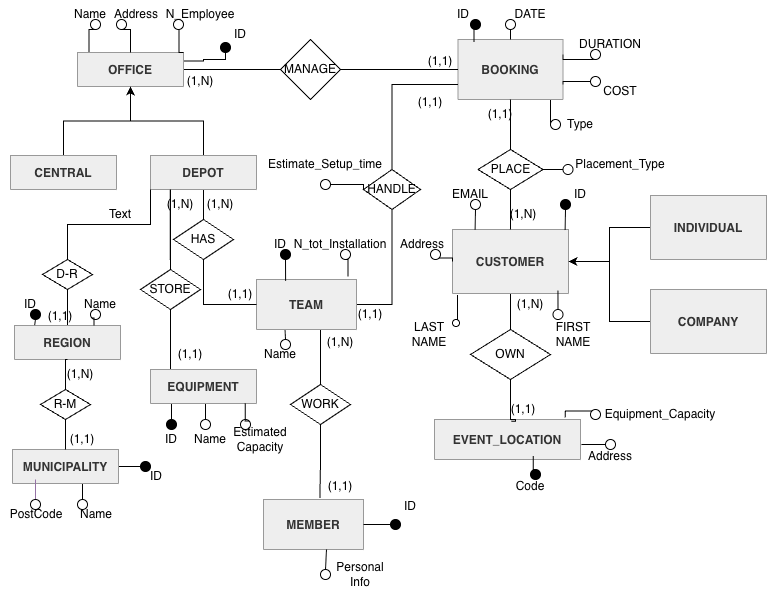
\includegraphics[width=0.95\textwidth]{uploads/ConceptualSchema-StageUP.drawio.png}
    }{%
        \fbox{\parbox{0.9\textwidth}{\centering Conceptual schema image not found at \texttt{uploads/ConceptualSchema-StageUP.drawio.png}.}}
    }
    \caption{Conceptual schema for the StageUp project.}
\end{figure}

The schema highlights the most important cardinalities and abstractions used throughout the report. In particular, it emphasizes the customer--location ownership relationship, the coordination role of offices, the territorial structure defined by regions and municipalities, and the operational role of teams in handling bookings and installations. This conceptual view serves as the bridge between the requirement analysis and the object-relational implementation discussed in the following sections.

\subsection{Conceptual-to-Implementation Alignment}
The project uses a mixed strategy (top-down plus bottom-up). The final implementation preserves core concepts while applying practical simplifications:
\begin{itemize}
    \item Customers are represented using a type discriminator (\texttt{CustomerType}) instead of subtype tables.
    \item Event locations are implemented with a global key (\texttt{LocationCode}).
    \item Booking coordination is represented via \texttt{HandledBy REF Office\_t} and operational assignment via \texttt{AssignedTeam REF Team\_t}.
\end{itemize}

\subsection{Data Dictionary}

\subsubsection*{Entities}
\begin{center}
\renewcommand{\arraystretch}{1.5}
\small
\begin{tabular}{|p{0.18\textwidth}|p{0.32\textwidth}|p{0.32\textwidth}|p{0.12\textwidth}|}
\hline
\rowcolor[rgb]{0.1, 0.3, 0.5} 
\textcolor{white}{\textbf{Entity}} & \textcolor{white}{\textbf{Description}} & \textcolor{white}{\textbf{Attributes}} & \textcolor{white}{\textbf{Identifier}} \\ \hline
\textbf{Office} & Generalization for company buildings (Central or Depot). & Name, Address (Street, StreetNo, ZipCode, City, Province), NoEmployees & Name \\ \hline
\textbf{Central Office} & Specialization of Office. Coordinates organization bookings. & - & (Name) \\ \hline
\textbf{Depot} & Specialization of Office. Manages local teams and regions. & - & (Name) \\ \hline
\textbf{Customer} & Actor requesting services. Can be Individual or Company. & CustomerCode, FirstName, LastName, Email, CustomerType, Address & CustomerCode \\ \hline
\textbf{Event Location} & Physical site for AV installation (Weak entity on Customer). & Code, Address, SetupTimeEstimate, EquipmentCapacity & Code \\ \hline
\textbf{Booking} & Service request for equipment rental and installation. & BookingID, Type, Date, Duration, TotalCost & BookingID \\ \hline
\textbf{Team} & Personnel group handling physical installation. & TeamCode, Name, N\_Total\_Installations, Members, RegionRef, OfficeRef & TeamCode \\ \hline
\textbf{Member} & Personnel belonging to a Setup Team. & TaxCode, FirstName, LastName, BirthDate & TaxCode \\ \hline
\textbf{Region} & Geographical area managed by a specific Depot. & Name & Name \\ \hline
\textbf{Municipality} & Local administrative subdivision within a Region. & PostCode, Name & PostCode \\ \hline
\end{tabular}
\end{center}

\subsubsection*{Relationships}
\begin{center}
\renewcommand{\arraystretch}{1.5}
\small
\begin{tabular}{|p{0.18\textwidth}|p{0.32\textwidth}|p{0.32\textwidth}|p{0.12\textwidth}|}
\hline
\rowcolor[rgb]{0.1, 0.3, 0.5} 
\textcolor{white}{\textbf{Relationship}} & \textcolor{white}{\textbf{Description}} & \textcolor{white}{\textbf{Entities Involved}} & \textcolor{white}{\textbf{Attributes}} \\ \hline
\textbf{Manage} & Links the Office to the bookings it coordinates. & Office (1,N) \newline Booking (1,1) & - \\ \hline
\textbf{Assign} & Associates a Setup Team with a specific Booking. & Team (1,N) \newline Booking (1,1) & - \\ \hline
\textbf{Own} & Links an Event Location to its owner Customer. & Customer (1,N) \newline Event Location (1,1) & - \\ \hline
\textbf{Has} & Links a Depot to the Setup Teams it manages. & Depot (1,N) \newline Team (1,1) & - \\ \hline
\textbf{Contains} & Relates a Team to its members as a bounded collection. & Team (1,1) \newline Member (0,10) & - \\ \hline
\textbf{D-R} & Associates a Depot with the Region in which it operates. & Depot (1,1) \newline Region (1,1) & - \\ \hline
\textbf{R-M} & Subdivides a Region into multiple Municipalities. & Region (1,1) \newline Municipality (1,N) & - \\ \hline
\textbf{Store} & Associates Office structures with Equipment storage and availability. & Office (1,N) \newline Equipment (1,N) & - \\ \hline
\end{tabular}
\end{center}

\subsection{Business Rules}

The following table reports the design intent and how each constraint has been technically implemented in the Oracle Object-Relational schema.

\begin{center}
\renewcommand{\arraystretch}{1.5}
\small
\begin{tabular}{|p{0.10\textwidth}|p{0.80\textwidth}|}
\hline
\rowcolor[rgb]{0.1, 0.3, 0.5} 
\textcolor{white}{\textbf{ID}} & \textcolor{white}{\textbf{Constraint Description}} \\ \hline

\textbf{BR1} & A Team can contain at most 10 Members; this rule is enforced through \texttt{VARRAY(10)} in \texttt{Member\_VA}. \\ \hline

\textbf{BR2} & Team territorial assignment is constrained by a single Region reference, enforced through \texttt{RegionRef} in \texttt{Team\_t} and \texttt{SCOPE FOR (RegionRef)}. \\ \hline

\textbf{BR3} & Booking total cost must be a strictly positive value, enforced through \texttt{CHECK (TotalCost > 0)} on \texttt{Booking\_TAB}. \\ \hline

\textbf{BR4} & Team operational count must be synchronized when bookings are inserted, deleted, or reassigned; this behavior is enforced through \texttt{TrgSyncTeamOps}, \texttt{ASSIGN\_TEAM\_TO\_BOOKING}, and the helper procedures \texttt{IncrementOperationsCount}/\texttt{DecrementOperationsCount}. \\ \hline

\textbf{BR5} & Customer and booking data must remain valid with respect to email format, dates, and booking-domain values; this is enforced through table-level \texttt{CHECK} constraints and \texttt{TrgBookingDates}. \\ \hline

\textbf{BR6} & Team members and event locations must remain consistent with the domain rules; this is enforced through \texttt{TrgTeamMemberDates}, \texttt{TrgTeamMustHaveMembers}, and table-level checks on \texttt{Location\_TAB}. \\ \hline

\textbf{BR7} & Promotional bookings are allowed only on locations with sufficient equipment capacity; this is enforced through \texttt{TrgCheckLocationCapacity}, which rejects \texttt{BookingType = 'Promotional'} when \texttt{EquipmentCapacity < 100}. \\ \hline

\end{tabular}
\end{center}

\section{Logical Design}

In the logical phase, it is essential to consider the operations required to restructure the ER diagram into an optimized system. This process involves analyzing the relationships and entities to ensure that the conceptual model is translated into a more efficient and performant structure for the Object-Relational Database.

\subsection{Operations}
Based on the system requirements, the following core operations define the daily workload of the StageUp Inc. database:

\begin{itemize}
    \item \textbf{(OP1)} Enter all data related to a new customer (10 times per day).
    \item \textbf{(OP2)} Record a new booking (300 times per day).
    \item \textbf{(OP3)} Register a new event location (50 times per day).
    \item \textbf{(OP4)} View the team that handled setups at a specific event location (20 times per day).
    \item \textbf{(OP5)} Print a list of event locations sorted in descending order by the number of bookings handled at each location (5 times per day).
\end{itemize}

\subsection{Table of Volumes and Operations}

Considering the specifications provided, the system manages an average of 100 setup teams, each with a maximum of 10 members (estimated average of 5 members per team). The company operates across 22 regions (the Italian territory including San Marino and the Vatican City), with one Depot assigned to manage each region. Assuming that each Depot operates on average in 10 municipalities, the system covers approximately 220 municipalities overall.

For the workload analysis, we assume a baseline dataset composed of \textbf{800 customers}, \textbf{1,000 event locations}, and \textbf{2,000 bookings}. The remaining structural volumes are kept consistent with the organizational assumptions of the project.

\vspace{0.5cm}

\noindent\textbf{Table of Volumes} \\
\renewcommand{\arraystretch}{1.15}
\small
\begin{tabularx}{\textwidth}{|Y|P{0.10\textwidth}|P{0.18\textwidth}|}
    \hline
    \rowcolor[rgb]{0.1, 0.3, 0.5}
    \textcolor{white}{\textbf{Concept}} & \textcolor{white}{\textbf{Type}} & \textcolor{white}{\textbf{Volume}} \\ \hline
    Office & E & 23 \\ \hline
    Central Office & E & 1 \\ \hline
    Depot & E & 22 \\ \hline
    Region & E & 22 \\ \hline
    Municipality & E & 220 \\ \hline
    Setup Team & E & 100 \\ \hline
    Member & E & 500 \\ \hline
    Equipment & E & 1,000 \\ \hline
    Customer & E & 800 \\ \hline
    Event Location & E & 1,000 \\ \hline
    Booking & E & 2,000 \\ \hline
    Manage (Office-Booking) & R & 2,000 \\ \hline
    Place (Customer-Booking) & R & 2,000 \\ \hline
    Own (Customer-Location) & R & 1,000 \\ \hline
    Handle (Booking-Team) & R & 2,000 \\ \hline
    Has (Depot-Team) & R & 100 \\ \hline
    Work (Team-Member) & R & 500 \\ \hline
    D-R (Depot-Region) & R & 22 \\ \hline
    R-M (Region-Muni.) & R & 220 \\ \hline
    Store (Office-Equipment) & R & 1,000 \\ \hline
\end{tabularx}

\vspace{0.5cm}

\noindent\textbf{Table of Operations} \\
\renewcommand{\arraystretch}{1.2}
\small
\begin{tabularx}{0.72\textwidth}{|Y|P{0.12\textwidth}|P{0.22\textwidth}|}
    \hline
    \rowcolor[rgb]{0.1, 0.3, 0.5}
    \textcolor{white}{\textbf{Operation}} & \textcolor{white}{\textbf{Type}} & \textcolor{white}{\textbf{Frequency}} \\ \hline
    Op 1 & I & 10 per day \\ \hline
    Op 2 & I & 300 per day \\ \hline
    Op 3 & I & 50 per day \\ \hline
    Op 4 & R & 20 per day \\ \hline
    Op 5 & R & 5 per day \\ \hline
\end{tabularx}
\vspace{0.5cm}

\subsection{Performance Analysis: Analysis of Redundancies}

To optimize the logical schema, we evaluate the redundant attribute \texttt{N\_Total\_Installations} associated with the \texttt{Team\_t} entity. We must verify if the storage and update costs are justified by the read performance gains.

We analyze two operations: 
\begin{itemize}
    \item \textbf{Operation 2 (OP2):} Record a new booking (Write operation, 300 times/day).
    \item \textbf{Ranking Operation:} View the team performance dashboard, which sorts teams by installations (Read operation, estimated 20 times/day).
\end{itemize}

\vspace{0.3cm}

\noindent\textbf{Access Table in the Presence of Redundancy} \\
\renewcommand{\arraystretch}{1.2}
\small
\begin{tabularx}{0.88\textwidth}{|Y|P{0.08\textwidth}|P{0.12\textwidth}|P{0.10\textwidth}|}
    \hline
    \rowcolor[rgb]{0.1, 0.3, 0.5}
    \textcolor{white}{\textbf{Concept}} & \textcolor{white}{\textbf{Type}} & \textcolor{white}{\textbf{Accesses}} & \textcolor{white}{\textbf{Mode}} \\ \hline
    \multicolumn{4}{|c|}{\cellcolor[rgb]{0.9, 0.9, 0.9}\textbf{OP2 (300/day)}} \\ \hline
    Booking & E & 1 & W \\ \hline
    Team & E & 1 & R \\ \hline
    Team & E & 1 & W \\ \hline
    \multicolumn{4}{|c|}{\textit{Cost per operation: 3 $\rightarrow$ Daily cost: 900}} \\ \hline
    \multicolumn{4}{|c|}{\cellcolor[rgb]{0.9, 0.9, 0.9}\textbf{Ranking (20/day)}} \\ \hline
    Team & E & 100 & R \\ \hline
    \multicolumn{4}{|c|}{\textit{Cost per operation: 100 $\rightarrow$ Daily cost: 2,000}} \\ \hline
    \multicolumn{3}{|r|}{\textbf{Total daily cost:}} & \textbf{2,900} \\ \hline
\end{tabularx}

\vspace{0.5cm}

\noindent\textbf{Access Table in the Absence of Redundancy} \\
\renewcommand{\arraystretch}{1.2}
\small
\begin{tabularx}{0.88\textwidth}{|Y|P{0.08\textwidth}|P{0.12\textwidth}|P{0.10\textwidth}|}
    \hline
    \rowcolor[rgb]{0.1, 0.3, 0.5}
    \textcolor{white}{\textbf{Concept}} & \textcolor{white}{\textbf{Type}} & \textcolor{white}{\textbf{Accesses}} & \textcolor{white}{\textbf{Mode}} \\ \hline
    \multicolumn{4}{|c|}{\cellcolor[rgb]{0.9, 0.9, 0.9}\textbf{OP2 (300/day)}} \\ \hline
    Booking & E & 1 & W \\ \hline
    \multicolumn{4}{|c|}{\textit{Cost per operation: 1 $\rightarrow$ Daily cost: 300}} \\ \hline
    \multicolumn{4}{|c|}{\cellcolor[rgb]{0.9, 0.9, 0.9}\textbf{Ranking (20/day)}} \\ \hline
    Team & E & 100 & R \\ \hline
    Booking & E & 2,000 & R \\ \hline
    \multicolumn{4}{|c|}{\textit{Cost per operation: 2,100 $\rightarrow$ Daily cost: 42,000}} \\ \hline
    \multicolumn{3}{|r|}{\textbf{Total daily cost:}} & \textbf{42,300} \\ \hline
\end{tabularx}
\vspace{0.5cm}

Considering all operations, the total number of accesses per day is \textbf{2,900} with redundancy, while in the absence of redundancy, the total increases to \textbf{42,300} accesses per day due to the repeated aggregation over 2,000 bookings. Given a minimal storage requirement of 4 bytes for an integer, the 100 teams require only 400 bytes of extra storage. Therefore, we \textbf{maintain the redundant data}.

\subsection{Removing Generalization}
The relational model does not allow for the direct, native representation of generalizations in a way that perfectly preserves pure ER semantics without trade-offs. 
\begin{itemize}
    \item \textbf{Customer Hierarchy:} We collapsed the \texttt{Individual} and \texttt{Company} specializations into the parent \texttt{Customer} entity. This decision is based on the fact that the majority of the workload (creating bookings) targets the parent entity. We introduced a \texttt{CustomerType} discriminator attribute.
    \item \textbf{Office Hierarchy:} Similarly, \texttt{Central Office} and \texttt{Depot} were merged into a single \texttt{Office} table with an \texttt{OfficeType} discriminator. This avoids expensive joins when traversing the territory and booking logic.
\end{itemize}

\subsection{Partitioning and Merging}
For partitioning and merging, there are no critical anomalies or specific operational bottlenecks that require horizontal or vertical partitioning of the tables at this scale.

\subsection{Selection of Primary Identifiers}
To ensure robust identification across the system:
\begin{itemize}
    \item \textbf{Booking:} Since a service request does not have a natural unique identifier, we introduced a surrogate key (\texttt{BookingID}) driven by an Oracle Sequence.
    \item \textbf{Customer and Team:} We utilized the \texttt{CustomerCode} and \texttt{TeamCode} alphanumeric/numeric sequences provided in the requirements.
\end{itemize}

\subsection{Object Relational Consideration}
The primary entities are mapped to specifically typed tables (\texttt{Customer\_TAB}, \texttt{Booking\_TAB}, \texttt{Team\_TAB}, and the related supporting tables). To optimize relationships and navigation:
\begin{itemize}
    \item \textbf{Typed tables:} The UML classes are materialized as dedicated object tables, including \texttt{Region\_TAB}, \texttt{Municipality\_TAB}, \texttt{Team\_TAB}, \texttt{Customer\_TAB}, \texttt{Location\_TAB}, and \texttt{Booking\_TAB}. Equipment is modeled as a relational support table (\texttt{Equipment\_TAB}).
    \item \textbf{REFs:} \texttt{Booking\_t.AtLocation}, \texttt{Booking\_t.HandledBy}, \texttt{Booking\_t.AssignedTeam}, and \texttt{Location\_t.OwnerRef} replace standard foreign keys. This object-oriented approach prevents dangling pointers through \texttt{SCOPE IS} clauses and allows navigation via \texttt{DEREF}.
\end{itemize}

\subsection{Translation into Logical Schema (UML)}
The following UML class diagram translates the final logical decisions into an Object-Relational structure. Reusable object types (such as \texttt{Address\_t}) are utilized as building blocks for the main entities, while references (REFs) handle the associations.

\begin{figure}[h!]
    \centering
    \IfFileExists{prism-uploads/UML_StageUP.drawio.png}{%
        \includegraphics[width=\textwidth]{prism-uploads/UML_StageUP.drawio.png}
    }{%
        \fbox{\parbox{0.9\textwidth}{\centering UML diagram not found at \texttt{prism-uploads/UML\_StageUP.drawio.png}.}}
    }
    \caption{Logical Object-Relational Schema (UML).}
\end{figure}
\section{Physical Design}
In this section, we focus on the physical design of the system, showing how the types identified in the logical schema are implemented in Oracle object-relational form. The goal is to translate the conceptual and logical structures into concrete types, tables, references, and constraints that are suitable for storage, querying, and application support.

\subsection{Types and tables definitions}

\begin{center}
\renewcommand{\arraystretch}{1.4}
\small
\begin{tabularx}{0.95\textwidth}{|Y|Y|}
\hline
\rowcolor[rgb]{0.1, 0.3, 0.5}
\textcolor{white}{\textbf{Type definition}} & \textcolor{white}{\textbf{Main attributes and role}} \\ \hline
\texttt{Address\_t} & Stores street, street number, zip code, city, and province; it is reused by offices, customers, and event locations. \\ \hline
\texttt{Office\_t} & Represents a company office with name, embedded address, employee count, and office type. \\ \hline
\texttt{Region\_t} & Represents a geographic region through a region code and region name. \\ \hline
\texttt{Municipality\_t} & Represents a municipality with code, name, zip code, and a \texttt{REF} to its region. \\ \hline
\texttt{Customer\_t} & Represents a customer with code, name fields, email, customer classification, and embedded address. \\ \hline
\texttt{Location\_t} & Represents an event location with code, embedded address, setup estimate, equipment capacity, and owner reference. \\ \hline
\texttt{Booking\_t} & Represents a booking with date, type, duration, total cost, placement mode, and \texttt{REF}s to location, office, and assigned team. \\ \hline
\texttt{Team\_t} & Represents an operational team with code, name, operation count, member varray, and references to its region and office. \\ \hline
\texttt{Member\_t} & Represents a team member with tax code, first name, last name, and birth date. \\ \hline
\end{tabularx}
\end{center}

\subsubsection*{Address\_t}
We first define the reusable support type \texttt{Address\_t}, used by offices, customers, and event locations.

\begin{verbatim}
CREATE OR REPLACE TYPE Address_t AS OBJECT (
    Street VARCHAR2(30),
    StreetNo VARCHAR2(5),
    ZipCode NUMBER(5),
    City VARCHAR2(30),
    Province VARCHAR2(5)
);
/
\end{verbatim}

These support types reduce repetition and make the physical schema closer to the UML design by encapsulating shared attributes in modular structures.

\subsubsection*{Office\_t, Region\_t and Municipality\_t}
The territorial and organizational part of the UML is implemented through office, region, and municipality object types. This allows us to represent both company buildings and the territory in which each depot operates.

\begin{verbatim}
CREATE OR REPLACE TYPE Office_t AS OBJECT (
    Name VARCHAR2(30),
    Location Address_t,
    NoEmployees NUMBER,
    OfficeType VARCHAR2(15)
);
/

CREATE OR REPLACE TYPE Region_t AS OBJECT (
    RegionCode NUMBER,
    RegionName VARCHAR2(30)
);
/

CREATE OR REPLACE TYPE Municipality_t AS OBJECT (
    MunicipalityCode NUMBER,
    MunicipalityName VARCHAR2(30),
    MunicipalityZipCode NUMBER(5),
    RegionRef REF Region_t
);
/
\end{verbatim}

This part of the design reflects the UML links among offices, regions, and municipalities, and materializes the territorial structure required by the business rules.

\subsubsection*{Customer\_t, Location\_t and Booking\_t}
The customer side of the model includes the customer profile, the owned event locations, and the booking object that centralizes the operational workflow.

\begin{verbatim}
CREATE OR REPLACE TYPE Customer_t AS OBJECT (
    CustomerCode VARCHAR2(10),
    FirstName VARCHAR2(50),
    LastName VARCHAR2(50),
    Email VARCHAR2(50),
    CustomerType VARCHAR2(15),
    Address Address_t
);
/

CREATE OR REPLACE TYPE Location_t AS OBJECT (
    LocationCode VARCHAR2(10),
    Address Address_t,
    SetupTimeEstimate NUMBER,
    EquipmentCapacity NUMBER,
    OwnerRef REF Customer_t
);
/

CREATE OR REPLACE TYPE Booking_t AS OBJECT (
    BookingID NUMBER,
    BookingType VARCHAR2(20),
    BookingDate DATE,
    Duration NUMBER,
    TotalCost NUMBER(10,2),
    PlacementMode VARCHAR2(15),
    AtLocation REF Location_t,
    HandledBy REF Office_t,
    AssignedTeam REF Team_t
);
/
\end{verbatim}

The use of \texttt{REF} attributes lets the booking object preserve the main logical associations of the UML diagram: the booking occurs at a location, is coordinated by an office, and is assigned to a team.

\subsubsection*{Team\_t and Member\_VA}
The operational execution layer is represented through teams and members. Members are stored as a bounded \texttt{VARRAY} directly inside each team, enforcing BR1 at schema level.

\begin{verbatim}
CREATE OR REPLACE TYPE Team_t AS OBJECT (
    TeamCode NUMBER,
    TeamName VARCHAR2(30),
    N_Total_Installations NUMBER,
    Members Member_VA,
    RegionRef REF Region_t,
    OfficeRef REF Office_t
);
/

CREATE OR REPLACE TYPE Member_t AS OBJECT (
    TaxCode CHAR(16),
    FirstName VARCHAR2(25),
    LastName VARCHAR2(25),
    BirthDate DATE
);
/
CREATE OR REPLACE TYPE Member_VA AS VARRAY(10) OF Member_t;
/
\end{verbatim}

Equipment availability is maintained in a relational support table (\texttt{Equipment\_TAB}) with non-negative stock checks.

\subsection{Table definitions and constraints}

\begin{center}
\renewcommand{\arraystretch}{1.4}
\small
\begin{tabularx}{0.95\textwidth}{|Y|Y|}
\hline
\rowcolor[rgb]{0.1, 0.3, 0.5}
\textcolor{white}{\textbf{Typed table}} & \textcolor{white}{\textbf{Key constraints and implementation notes}} \\ \hline
\texttt{Office\_TAB} & Typed table of \texttt{Office\_t}; primary key on name and a domain check on \texttt{OfficeType}. \\ \hline
\texttt{Region\_TAB} & Typed table of \texttt{Region\_t}; primary key on \texttt{RegionCode} and mandatory region name. \\ \hline
\texttt{Municipality\_TAB} & Typed table of \texttt{Municipality\_t}; primary key on municipality code and mandatory scoped region reference. \\ \hline
\texttt{Customer\_TAB} & Typed table of \texttt{Customer\_t}; primary key on customer code, mandatory email, and a domain check on customer type. \\ \hline
\texttt{Location\_TAB} & Typed table of \texttt{Location\_t}; primary key on location code, mandatory scoped owner reference, and positive setup/capacity checks. \\ \hline
\texttt{Team\_TAB} & Typed table of \texttt{Team\_t}; primary key on team code, default operation counter, member varray, and scoped references to region and office. \\ \hline
\texttt{Equipment\_TAB} & Relational support table; primary key on item code and non-negative unit availability. \\ \hline
\texttt{Booking\_TAB} & Typed table of \texttt{Booking\_t}; primary key on booking ID, mandatory operational attributes, scoped references, and checks on booking type, placement mode, and total cost. \\ \hline
\end{tabularx}
\end{center}

\subsubsection*{Territorial and master tables}
We now map the main structural types into typed tables and add primary-key and domain constraints where required.

\begin{verbatim}
CREATE TABLE Office_TAB OF Office_t (
    Name PRIMARY KEY,
    OfficeType NOT NULL,
    CHECK (OfficeType IN ('Central', 'Depot'))
);
/

CREATE TABLE Region_TAB OF Region_t (
    RegionCode PRIMARY KEY,
    RegionName NOT NULL
);
/

CREATE TABLE Municipality_TAB OF Municipality_t (
    MunicipalityCode PRIMARY KEY,
    RegionRef NOT NULL,
    SCOPE FOR (RegionRef) IS Region_TAB
);
/

CREATE TABLE Customer_TAB OF Customer_t (
    CustomerCode PRIMARY KEY,
    Email NOT NULL,
    CustomerType NOT NULL,
    CHECK (REGEXP_LIKE(Email, '^[A-Za-z0-9._%+-]+@[A-Za-z0-9.-]+\.[A-Za-z]{2,}$')),
    CHECK (CustomerType IN ('Individual', 'Company'))
);
/

CREATE TABLE Location_TAB OF Location_t (
    LocationCode PRIMARY KEY,
    OwnerRef NOT NULL,
    SetupTimeEstimate NOT NULL,
    EquipmentCapacity NOT NULL,
    CHECK (SetupTimeEstimate > 0),
    CHECK (EquipmentCapacity > 0),
    SCOPE FOR (OwnerRef) IS Customer_TAB
);
/
\end{verbatim}

These typed tables implement the stable master data of the application. The \texttt{SCOPE IS} clauses restrict references to the intended object tables and improve integrity and navigation performance.

\subsubsection*{Operational tables}
The operational tables support installations, equipment storage, and booking execution, and contain the dynamic data used most frequently by the application.

\begin{verbatim}
CREATE TABLE Team_TAB OF Team_t (
    TeamCode PRIMARY KEY,
    TeamName NOT NULL,
    N_Total_Installations DEFAULT 0 NOT NULL,
    RegionRef NOT NULL,
    OfficeRef NOT NULL,
    SCOPE FOR (RegionRef) IS Region_TAB,
    SCOPE FOR (OfficeRef) IS Office_TAB
);
/

CREATE TABLE Equipment_TAB (
    ItemCode NUMBER PRIMARY KEY,
    Description VARCHAR2(100),
    UnitsAvailable NOT NULL,
    CHECK (UnitsAvailable >= 0)
);
/

CREATE TABLE Booking_TAB OF Booking_t (
    BookingID PRIMARY KEY,
    BookingType NOT NULL,
    BookingDate NOT NULL,
    Duration NOT NULL,
    TotalCost NOT NULL,
    PlacementMode NOT NULL,
    AtLocation NOT NULL,
    HandledBy NOT NULL,
    AssignedTeam NOT NULL,
    SCOPE FOR (AtLocation) IS Location_TAB,
    SCOPE FOR (HandledBy) IS Office_TAB,
    SCOPE FOR (AssignedTeam) IS Team_TAB,
    CHECK (BookingType IN ('One-time', 'Recurring', 'Seasonal', 'Promotional')),
    CHECK (PlacementMode IN ('Phone', 'Mail', 'Email', 'Website')),
    CHECK (TotalCost > 0)
);
/
\end{verbatim}

This group of tables materializes the most relevant UML associations. In particular, \texttt{Booking\_TAB} acts as the central operational table and links together event locations, handling offices, and assigned teams through typed object references.

\subsection{Trigger Implementation and Validation Tests}
To fully enforce the business rules at database level, the project includes a dedicated trigger module (\texttt{scripts/04\_triggers.sql}) and a companion test campaign (\texttt{scripts/07\_triggertests.sql}).
In this report section, we list only the triggers used for synchronization and domain validation.

\subsubsection*{Trigger Catalog}
The following triggers are implemented and actively used by the application:
\begin{itemize}
    \item \texttt{TrgSyncTeamOps} (AFTER INSERT/DELETE/UPDATE OF \texttt{HandledBy} on \texttt{Booking\_TAB}): keeps team installation counters synchronized when bookings are inserted, reassigned, or deleted.
    \item \texttt{TrgTeamMemberDates} (BEFORE INSERT/UPDATE OF \texttt{Members} on \texttt{Team\_TAB}): rejects null/future birth dates in member collections.
    \item \texttt{TrgBookingDates} (BEFORE INSERT/UPDATE OF \texttt{BookingDate} on \texttt{Booking\_TAB}): blocks bookings in the past (except controlled bootstrap population).
    \item \texttt{TrgCheckLocationCapacity} (BEFORE INSERT/UPDATE OF \texttt{AtLocation}, \texttt{BookingType} on \texttt{Booking\_TAB}): rejects promotional bookings when location capacity is below threshold.
    \item \texttt{TrgTeamMustHaveMembers} (BEFORE INSERT/UPDATE OF \texttt{Members} on \texttt{Team\_TAB}): enforces non-empty teams.
\end{itemize}

This implementation directly supports BR1, BR4, BR5, BR6, and BR7 from the business-rule table and complements table-level \texttt{CHECK} constraints.

\subsubsection*{SQL Code Triggers)}
For completeness, we report the core SQL definitions of the real \texttt{Trg*} triggers used in the project.

\begin{verbatim}
CREATE OR REPLACE TRIGGER TrgSyncTeamOps
AFTER INSERT OR DELETE OR UPDATE OF HandledBy ON Booking_TAB
FOR EACH ROW
DECLARE
    v_new_team_code NUMBER;
    v_old_team_code NUMBER;
BEGIN
    IF INSERTING THEN
        SELECT t.TeamCode INTO v_new_team_code
        FROM Team_TAB t
        WHERE REF(t) = :NEW.AssignedTeam;
        IncrementOperationsCount(v_new_team_code);
    END IF;

    IF DELETING THEN
        SELECT t.TeamCode INTO v_old_team_code
        FROM Team_TAB t
        WHERE REF(t) = :OLD.AssignedTeam;
        DecrementOperationsCount(v_old_team_code);
    END IF;

    IF UPDATING THEN
        SELECT t.TeamCode INTO v_old_team_code
        FROM Team_TAB t
        WHERE REF(t) = :OLD.AssignedTeam;
        SELECT t.TeamCode INTO v_new_team_code
        FROM Team_TAB t
        WHERE REF(t) = :NEW.AssignedTeam;
        DecrementOperationsCount(v_old_team_code);
        IncrementOperationsCount(v_new_team_code);
    END IF;
END TrgSyncTeamOps;
/
\end{verbatim}

\begin{verbatim}
CREATE OR REPLACE TRIGGER TrgTeamMemberDates
BEFORE INSERT OR UPDATE OF Members ON Team_TAB
FOR EACH ROW
DECLARE
    v_index PLS_INTEGER;
BEGIN
    IF :NEW.Members IS NOT NULL THEN
        v_index := :NEW.Members.FIRST;
        WHILE v_index IS NOT NULL LOOP
            IF :NEW.Members(v_index).BirthDate IS NULL
               OR :NEW.Members(v_index).BirthDate > TRUNC(SYSDATE) THEN
                RAISE_APPLICATION_ERROR(-20990,
                    'Team member birth date cannot be NULL or in the future');
            END IF;
            v_index := :NEW.Members.NEXT(v_index);
        END LOOP;
    END IF;
END;
/
\end{verbatim}

\begin{verbatim}
CREATE OR REPLACE TRIGGER TrgBookingDates
BEFORE INSERT OR UPDATE OF BookingDate ON Booking_TAB
FOR EACH ROW
BEGIN
    IF SYS_CONTEXT('USERENV', 'CLIENT_IDENTIFIER') = 'BOOTSTRAP_POPULATION' THEN
        RETURN;
    END IF;

    IF :NEW.BookingDate < TRUNC(SYSDATE) THEN
        RAISE_APPLICATION_ERROR(-20992, 'Booking date cannot be in the past');
    END IF;
END;
/
\end{verbatim}

\begin{verbatim}
CREATE OR REPLACE TRIGGER TrgCheckLocationCapacity
BEFORE INSERT OR UPDATE OF AtLocation, BookingType ON Booking_TAB
FOR EACH ROW
DECLARE
    v_loc_capacity NUMBER;
BEGIN
    SELECT l.EquipmentCapacity INTO v_loc_capacity
    FROM Location_TAB l
    WHERE REF(l) = :NEW.AtLocation;

    IF :NEW.BookingType = 'Promotional' AND v_loc_capacity < 100 THEN
        RAISE_APPLICATION_ERROR(-20985,
            'Venue capacity is too low for a Promotional setup.');
    END IF;
END;
/
\end{verbatim}

\begin{verbatim}
CREATE OR REPLACE TRIGGER TrgTeamMustHaveMembers
BEFORE INSERT OR UPDATE OF Members ON Team_TAB
FOR EACH ROW
BEGIN
    IF :NEW.Members IS NULL OR :NEW.Members.COUNT = 0 THEN
        RAISE_APPLICATION_ERROR(-20995,
            'A team must contain at least one member');
    END IF;
END;
/
\end{verbatim}

\subsubsection*{Trigger Test Campaign (A--K)}
The validation suite in \texttt{scripts/07\_triggertests.sql} executes positive and negative checks with automatic identifiers and transactional cleanup. Focusing only on triggers, the relevant outcomes are:
\begin{itemize}
    \item \textbf{Tests B/C/D}: verify \texttt{TrgSyncTeamOps} synchronization semantics on booking \texttt{INSERT}, \texttt{UPDATE HandledBy}, and \texttt{DELETE}.
    \item \textbf{Test F}: verifies \texttt{TrgTeamMemberDates} rejects future birth dates.
    \item \textbf{Test H}: verifies \texttt{TrgBookingDates} rejects bookings in the past.
    \item \textbf{Test J}: verifies \texttt{TrgTeamMustHaveMembers} rejects empty member collections.
    \item \textbf{Test K}: verifies \texttt{TrgCheckLocationCapacity} rejects promotional bookings on low-capacity locations.
\end{itemize}

At the end of the test script, a final snapshot reports: total teams, total bookings, and bookings without assigned team. This provides a consistency checkpoint after test execution and confirms that assignment/synchronization triggers preserve operational integrity.

\subsubsection*{SQL Code Extracts (Trigger Tests)}
The following excerpts show the effective structure of the trigger-focused tests.

\begin{verbatim}
-- TEST B/C/D: TrgSyncTeamOps
INSERT INTO Booking_TAB (..., HandledBy) VALUES (..., v_office_ref_1);
-- expected: Team A operations +1

UPDATE Booking_TAB SET HandledBy = v_office_ref_2 WHERE BookingID = v_booking_id;
-- expected: Team A -1, Team B +1

DELETE FROM Booking_TAB WHERE BookingID = v_booking_id;
-- expected: Team B -1
\end{verbatim}

\begin{verbatim}
-- TEST F: TrgTeamMemberDates
INSERT INTO Team_TAB (..., Members, ...)
VALUES (..., Member_VA(Member_t('FUTURE1111111111','Future','Member',TRUNC(SYSDATE)+1)), ...);
-- expected: ORA error (future birth date rejected)
\end{verbatim}

\begin{verbatim}
-- TEST H: TrgBookingDates
INSERT INTO Booking_TAB (..., BookingDate, ...)
VALUES (..., TRUNC(SYSDATE)-1, ...);
-- expected: ORA error (past booking date rejected)
\end{verbatim}

\begin{verbatim}
-- TEST J: TrgTeamMustHaveMembers
INSERT INTO Team_TAB (..., Members, ...)
VALUES (..., Member_VA(), ...);
-- expected: ORA error (empty team rejected)
\end{verbatim}

\begin{verbatim}
-- TEST K: TrgCheckLocationCapacity
INSERT INTO Location_TAB (..., EquipmentCapacity, ...) VALUES (..., 50, ...);
INSERT INTO Booking_TAB (..., BookingType, AtLocation, ...)
VALUES (..., 'Promotional', (SELECT REF(l) FROM Location_TAB l WHERE ...), ...);
-- expected: ORA error (capacity < 100 for Promotional booking)
\end{verbatim}

\subsection{Qualitative Assessment: Indexes}

In this paragraph, we will choose specific indexing strategies based on the queries required to retrieve data for the system's core operations.

\begin{table}[h!]
    \centering
    \small
    \begin{tabular}{|l|p{0.8\textwidth}|}
        \hline
        \rowcolor[rgb]{0.1, 0.3, 0.5} 
        \textcolor{white}{\textbf{ID}} & \textcolor{white}{\textbf{Operation Description}} \\ \hline
        \textbf{(OP4)} & View the team that handled setups at a specific event location (20 times per day). \\ \hline
        \textbf{(OP5)} & Print a list of event locations sorted in descending order by the number of bookings handled (5 times per day). \\ \hline
    \end{tabular}
\end{table}

\subsubsection*{Operation 4}

Operation 4 requires retrieving specific records based on the event location where a booking took place. Due to our Object-Relational design, the BookingTable contains a REF pointer (Location\_Ref) pointing to the LocationTable.
If we do not index this REF column, the database will be forced to perform a Full Table Scan on all 2,000 bookings every time a user wants to view the history of a specific location. Since the query requires joining the exact location with the bookings and subsequently with the TeamTable, a direct access approach is preferred.
The optimized access path starts from a Hash Cluster lookup on the event location's address, and then joins the matching rows using the Location\_Ref as a search key on BookingTable. In practice, Oracle can use a B+Tree index on the Location\_Ref column to avoid a full scan of BookingTable. We also keep an index on Team\_Ref to support the subsequent navigation toward TeamTable when the application needs the full team details.

\begin{figure}[h!]
    \centering
    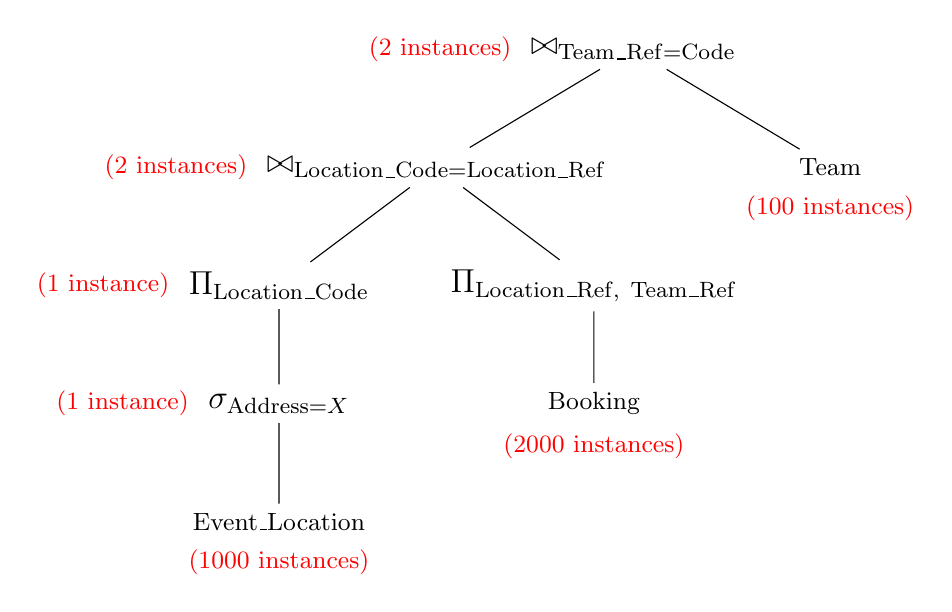
\begin{tikzpicture}[
        op/.style={font=\large},
        note/.style={font=\small},
        level 1/.style={sibling distance=5cm},
        level 2/.style={sibling distance=4cm},
        level 3/.style={sibling distance=3cm}
    ]

        \node[op, label={[red, font=\small]left:(2 instances)}] (join1) {$\bowtie_{\mathrm{Team\_Ref} = \mathrm{Code}}$}
            child {
                node[op, label={[red, font=\small]left:(2 instances)}] (join2) {$\bowtie_{\mathrm{Location\_Code} = \mathrm{Location\_Ref}}$}
                    child {
                        node[op, label={[red, font=\small]left:(1 instance)}] (piLoc) {$\Pi_{\mathrm{Location\_Code}}$}
                            child {
                                node[op, label={[red, font=\small]left:(1 instance)}] (sigmaLoc) {$\sigma_{\mathrm{Address} = X}$}
                                    child {
                                        node[note, label={[red, font=\small]below:(1000 instances)}] (locTab) {Event\_Location}
                                    }
                            }
                    }
                    child {
                        node[op] (piBkg) {$\Pi_{\mathrm{Location\_Ref,\ Team\_Ref}}$}
                            child {
                                node[note, label={[red, font=\small]below:(2000 instances)}] (bkgTab) {Booking}
                            }
                    }
            }
            child {
                node[note, label={[red, font=\small]below:(100 instances)}] (teamTab) {Team}
            };

    \end{tikzpicture}
    \caption{Phisycal Query Plan for Operation 4}
\end{figure}

The optimized access path starts from the location reference used as a search key on \texttt{Booking\_TAB(AtLocation)} and then projects the \texttt{AssignedTeam} reference for the matching rows. In practice, Oracle can use a B+Tree index on the \texttt{AtLocation} \texttt{REF} column to avoid a full scan of \texttt{Booking\_TAB}. We also keep an index on \texttt{AssignedTeam} to support the subsequent navigation or join toward \texttt{Team\_TAB} when the application needs the full team details.

\begin{verbatim}
-- Indexes on REF columns to optimize OP4 navigation
CREATE INDEX IDX_BOOKING_LOCATION ON BookingTable (Location_Ref);
CREATE INDEX IDX_BOOKING_TEAM ON BookingTable (Team_Ref);
CREATE INDEX IDX_BOOKING_CUSTOMER ON BookingTable (Customer_Ref);
\end{verbatim}

\subsubsection*{Operation 5}

In the given scenario, Operation 5 requires retrieving teams (or locations) ordered by their performance metrics (e.g., the redundant attribute \texttt{N\_Total\_Installations} in the \texttt{Team\_TAB}). Since this operation relies heavily on sorting (\texttt{ORDER BY N\_Total\_Installations DESC}), the goal is to optimize the retrieval of records based on this specific attribute.

\begin{figure}[h!]
    \centering
    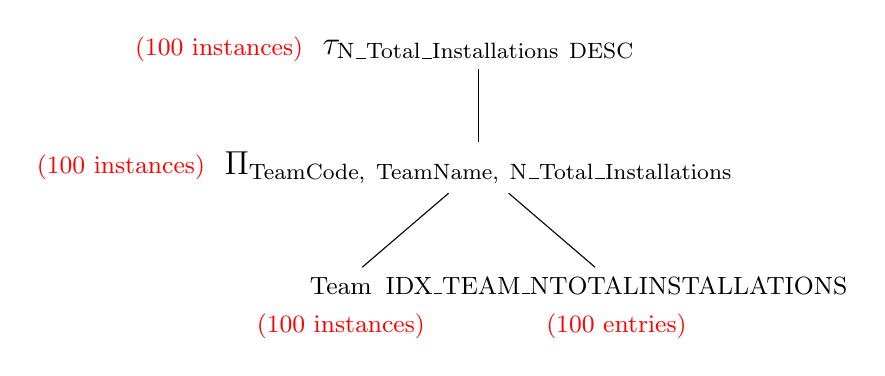
\begin{tikzpicture}[
        op/.style={font=\large},
        note/.style={font=\small},
        level 1/.style={sibling distance=4.5cm},
        level 2/.style={sibling distance=3.5cm}
    ]

        \node[op, label={[red, font=\small]left:(100 instances)}] (tau) {$\tau_{\mathrm{N\_Total\_Installations\ DESC}}$}
            child {
                node[op, label={[red, font=\small]left:(100 instances)}] (pi) {$\Pi_{\mathrm{TeamCode,\ TeamName,\ N\_Total\_Installations}}$}
                    child {
                        node[note, label={[red, font=\small]below:(100 instances)}] (teamTab) {Team}
                    }
                    child {
                        node[note, label={[red, font=\small]below:(100 entries)}] (idxTab) {IDX\_TEAM\_NTOTALINSTALLATIONS}
                    }
            };

    \end{tikzpicture}
    \caption{Phisycal Query Plan for Operation 5}
\end{figure}

A B+Tree index on the \texttt{N\_Total\_Installations} attribute is particularly well-suited for this type of operation. B+Tree indexes are highly efficient for range queries and sorting. By maintaining a balanced tree structure, the database can traverse the leaf entries in descending order and retrieve the teams in the desired order, bypassing the need for an expensive sort over the entire table.

The optimized access path therefore starts from the index on \texttt{Team\_TAB(N\_Total\_Installations)} and projects the attributes needed by the report. On the other hand, hash-based indexing techniques are primarily designed for equality lookups (exact matches). Because they do not preserve the inherent ordering of the data, a hash cluster cannot be leveraged effectively for operations that require sorting, such as the \texttt{ORDER BY} clause in OP5.

\begin{verbatim}
-- B+Tree index to optimize the sorting required by OP5
CREATE INDEX IdxTeamNTotalInstallations ON Team_TAB(N_Total_Installations);

-- Additional categorical indexes for reporting filters
CREATE INDEX IdxBookingType ON Booking_TAB(BookingType);
CREATE INDEX IdxBookingPlacement ON Booking_TAB(PlacementMode);
CREATE INDEX IdxOfficeType ON Office_TAB(OfficeType);
\end{verbatim}
\subsection{Views and ORDBMS Querying}
Implemented views include:
\begin{itemize}
    \item \texttt{ViewRegionMunicipalities}: territorial mapping between regions and municipalities.
    \item \texttt{ViewTeamMembers}: team-member expansion through \texttt{TABLE(CAST(Members AS Member\_VA))}.
    \item \texttt{ViewCustomerLocations}: customer-owned event locations with flattened address fields.
    \item \texttt{ViewBookingDetails}: chained \texttt{DEREF} navigation from booking to location, customer owner, handling office, and assigned team.
    \item \texttt{ViewCompanyOffices}: company offices and depots with location details.
    \item \texttt{ViewCentralOfficeBookings}: booking subset handled by the central office.
    \item \texttt{ViewDepotTeamAssignments}: team allocation by depot and region.
    \item \texttt{ViewCustomerActivity}: aggregate analytics by customer based on \texttt{ViewBookingDetails}.
\end{itemize}

\section{Architecture and Deployment}

The system is designed with a three-tier architecture to ensure modularity, scalability, and ease of deployment. The interaction between the front-end user interface and the back-end storage is managed through a containerized environment.

\subsection{Architecture Overview}
The application architecture consists of three primary components:
\begin{itemize}
    \item \textbf{Presentation Layer (Client):} A web-based interface accessed via a browser. It renders the Streamlit widgets and captures user interactions.
    \item \textbf{Application Layer (Streamlit Server):} Built with Python, this layer acts as the controller. it handles logic, manages session states, and communicates with the database using the \texttt{python-oracledb} driver. It transforms user inputs into Object-Relational SQL queries.
    \item \textbf{Data Layer (ORDBMS Server):} An Oracle Database instance that stores all Object Types, Typed Tables, and Triggers. It ensures data integrity and executes the business logic defined in the physical design.
\end{itemize}

\subsection{Deployment Diagram}
The deployment of the StageUp Inc. system is managed through \textbf{Docker} container technology. This ensures that the application and database environments remain isolated and reproducible.

\begin{figure}[H]
    \centering
    \IfFileExists{prism-uploads/architecture.drawio.png}{%
        \includegraphics[width=0.9\textwidth,height=0.72\textheight,keepaspectratio]{prism-uploads/architecture.drawio.png}
    }{%
        \fbox{\parbox{0.9\textwidth}{\centering Deployment diagram not found at \texttt{prism-uploads/architecture.drawio.png}.}}
    }
    \caption{UML Deployment Diagram for the StageUp system.}
\end{figure}

The diagram illustrates the network communication between the two main Docker nodes. The Application Server sends SQL requests over \textbf{TCP/IP} using a \textbf{JDBC/Oracle-Net} connection to the Database Server. Persistent storage is managed via a Docker Volume to ensure data is not lost when the container is restarted.

\section{GUI Screens}

The following interfaces encapsulate the main concepts of the StageUp system. The Streamlit platform provides a practical front-end through which different stakeholders can interact with the Oracle object-relational database without requiring direct SQL knowledge. The application is organized into three main functional viewpoints, aligned with the operational requirements discussed throughout the project.

\subsection{Customer View}
The customer-oriented interfaces group the workflows used by office personnel to manage the lifecycle of a client. The platform supports the registration of new customer profiles, whether \textbf{Individual} or \textbf{Company}, together with the generation of the corresponding unique customer code.

Once a customer has been selected, the operator can manage the related \textbf{Event Locations}. The interface supports the insertion of new physical sites while ensuring that address data and technical attributes, such as setup time and equipment capacity, are properly defined. In the same area of the application, the operator can also record \textbf{New Bookings}: the system generates a unique booking identifier and links the booking metadata to the selected customer, the chosen location, and the operational history already stored in the database.

\begin{figure}[H]
    \centering
    \IfFileExists{images/streamlit_customer_view_overview.png}{%
        \includegraphics[width=0.92\textwidth]{images/streamlit_customer_view_overview.png}
    }{%
        \fbox{\parbox{0.85\textwidth}{\centering Insert screenshot: Customer View Overview}}
    }
    \caption{Customer-view overview page used to browse core tables and operational records.}
\end{figure}

\subsubsection{Operation 1: Register New Customer}
This interface is used to create a new customer profile and automatically generate the corresponding unique identifier. The operator can choose whether the customer is an individual or a company and fill in the required personal or fiscal information together with the main contact details.

\begin{figure}[H]
    \centering
    \IfFileExists{images/streamlit_op1_register_customer.png}{%
        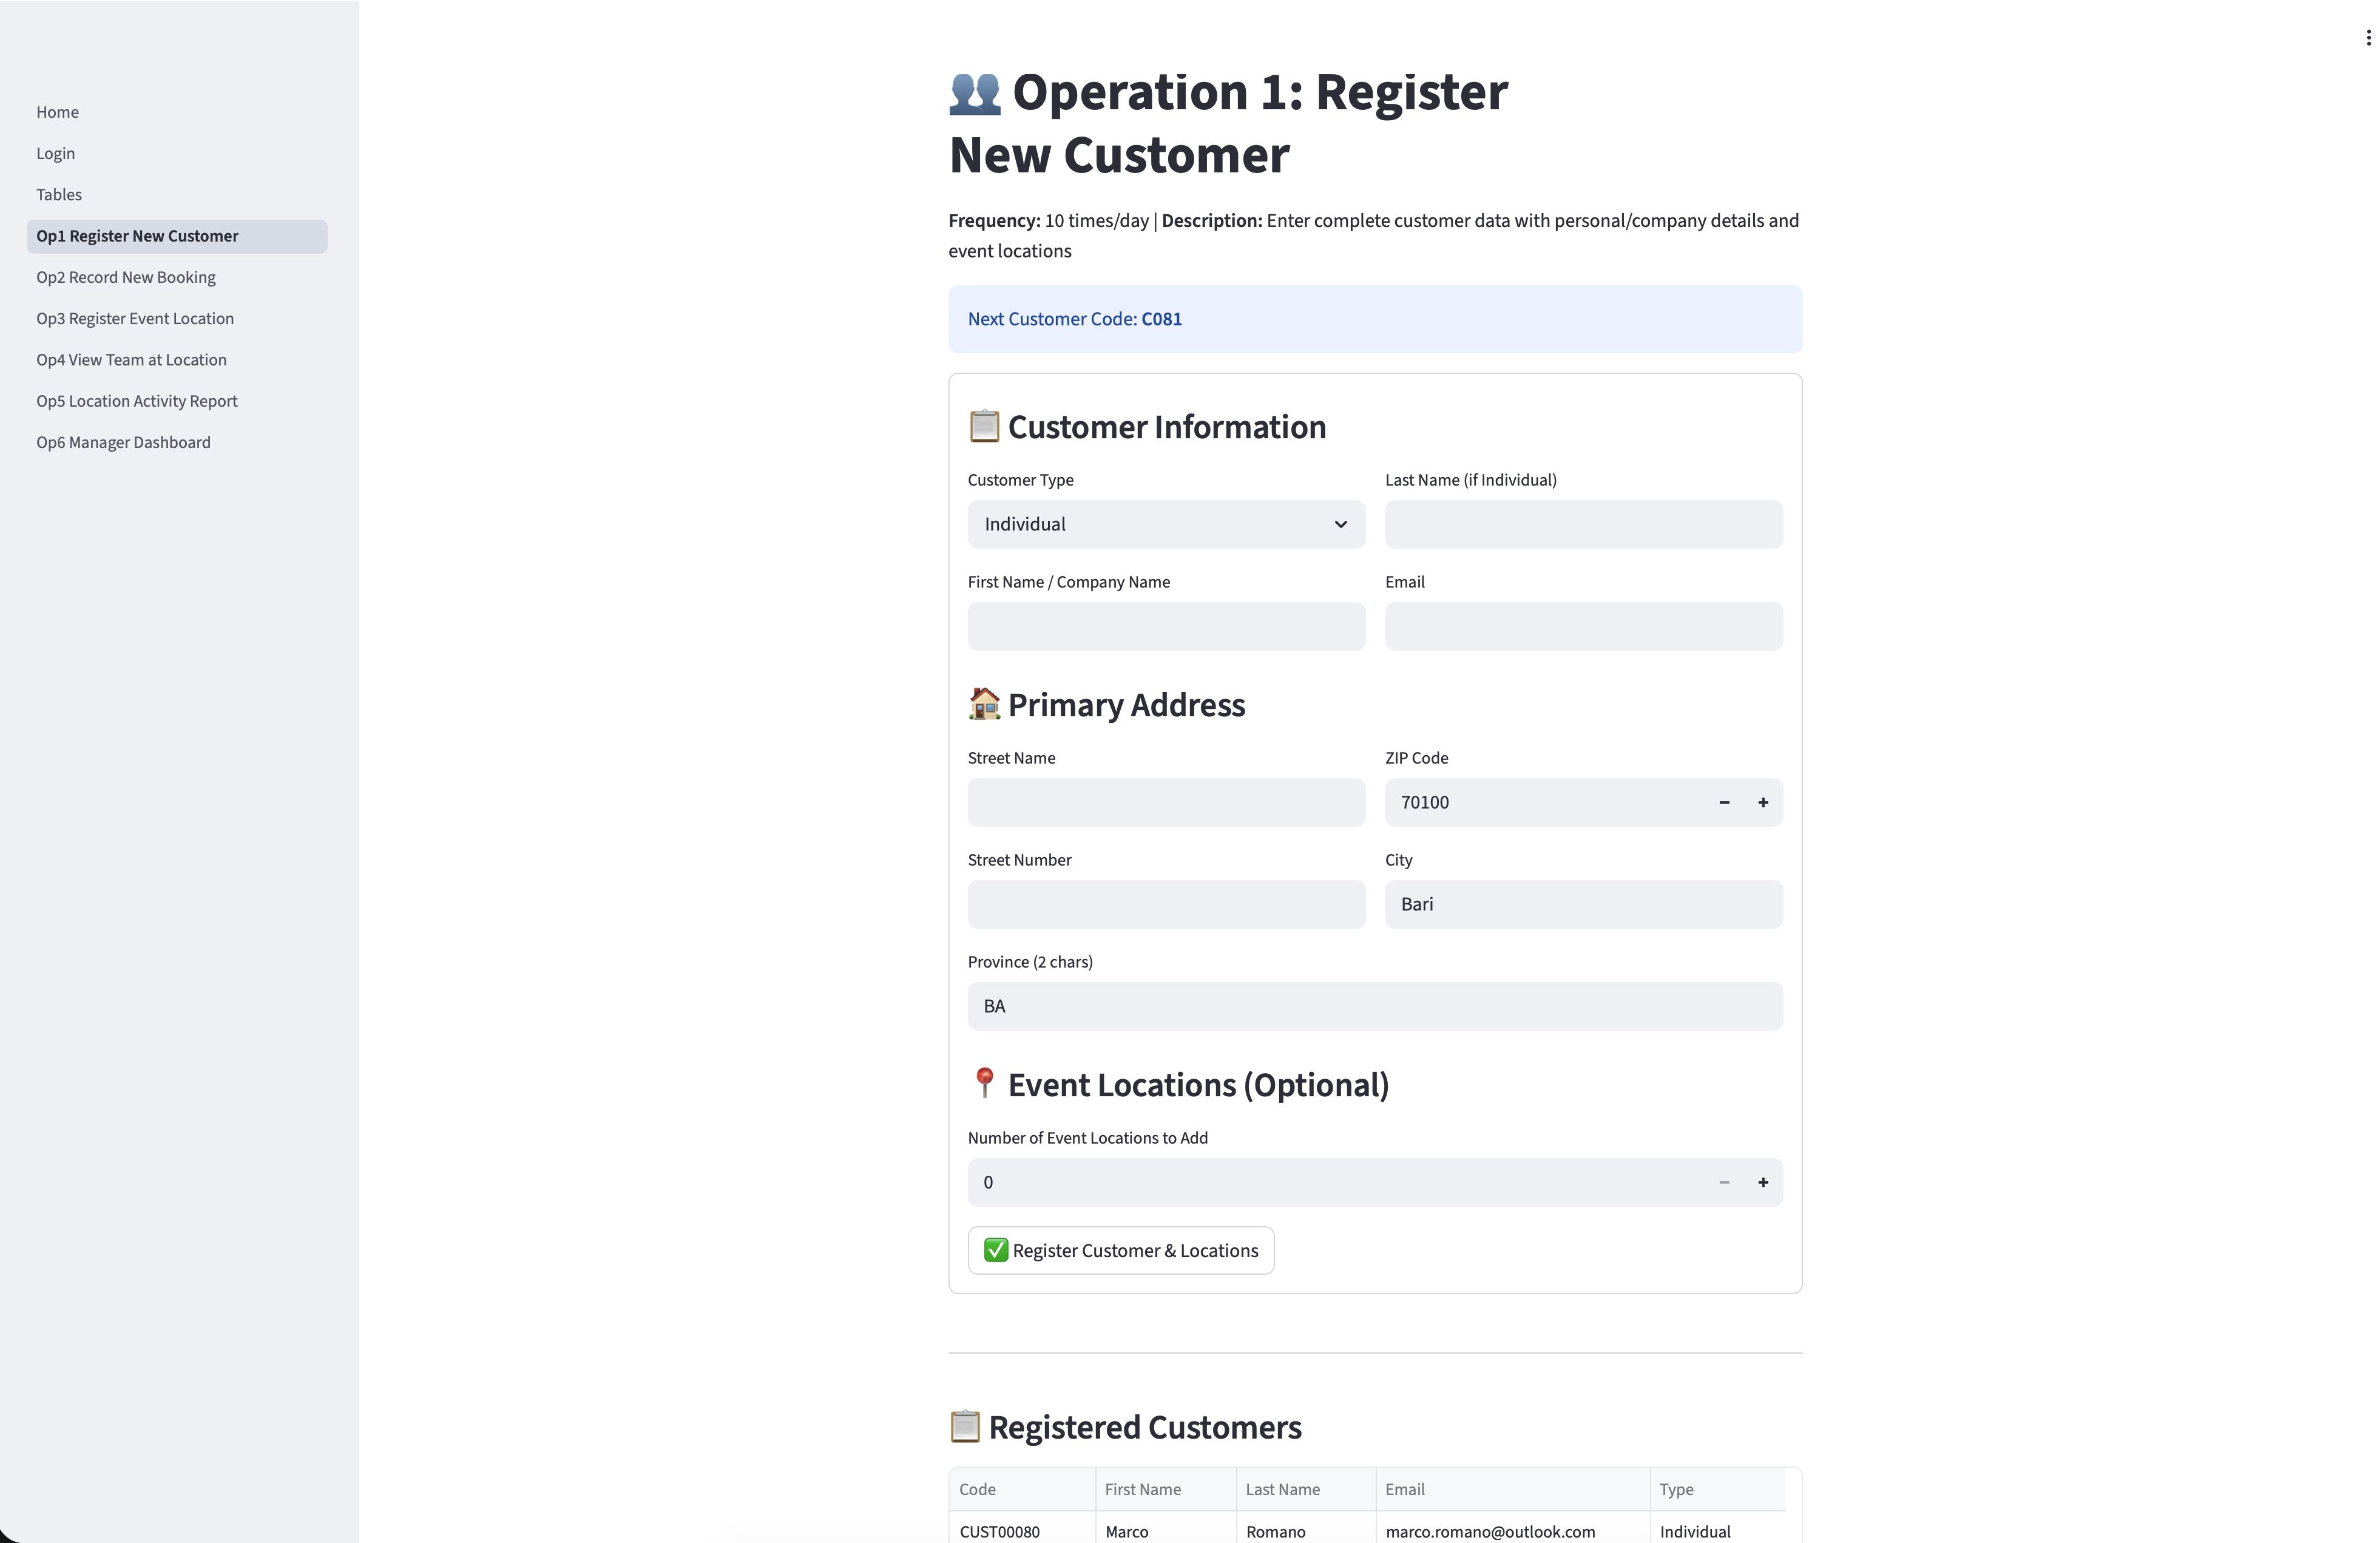
\includegraphics[width=0.72\textwidth]{images/streamlit_op1_register_customer.png}
    }{%
        \fbox{\parbox{0.8\textwidth}{\centering Insert screenshot: Operation 1 - Register New Customer}}
    }
    \caption{Interface for customer registration.}
\end{figure}

\subsubsection{Operation 2: Record New Booking}
This page allows office personnel to register a booking for a previously selected customer and event location. The form collects the service category, scheduling details, duration, cost, and team assignment so that each booking is fully connected to the operational database.

\begin{figure}[H]
    \centering
    \IfFileExists{images/streamlit_op2_record_booking.png}{%
        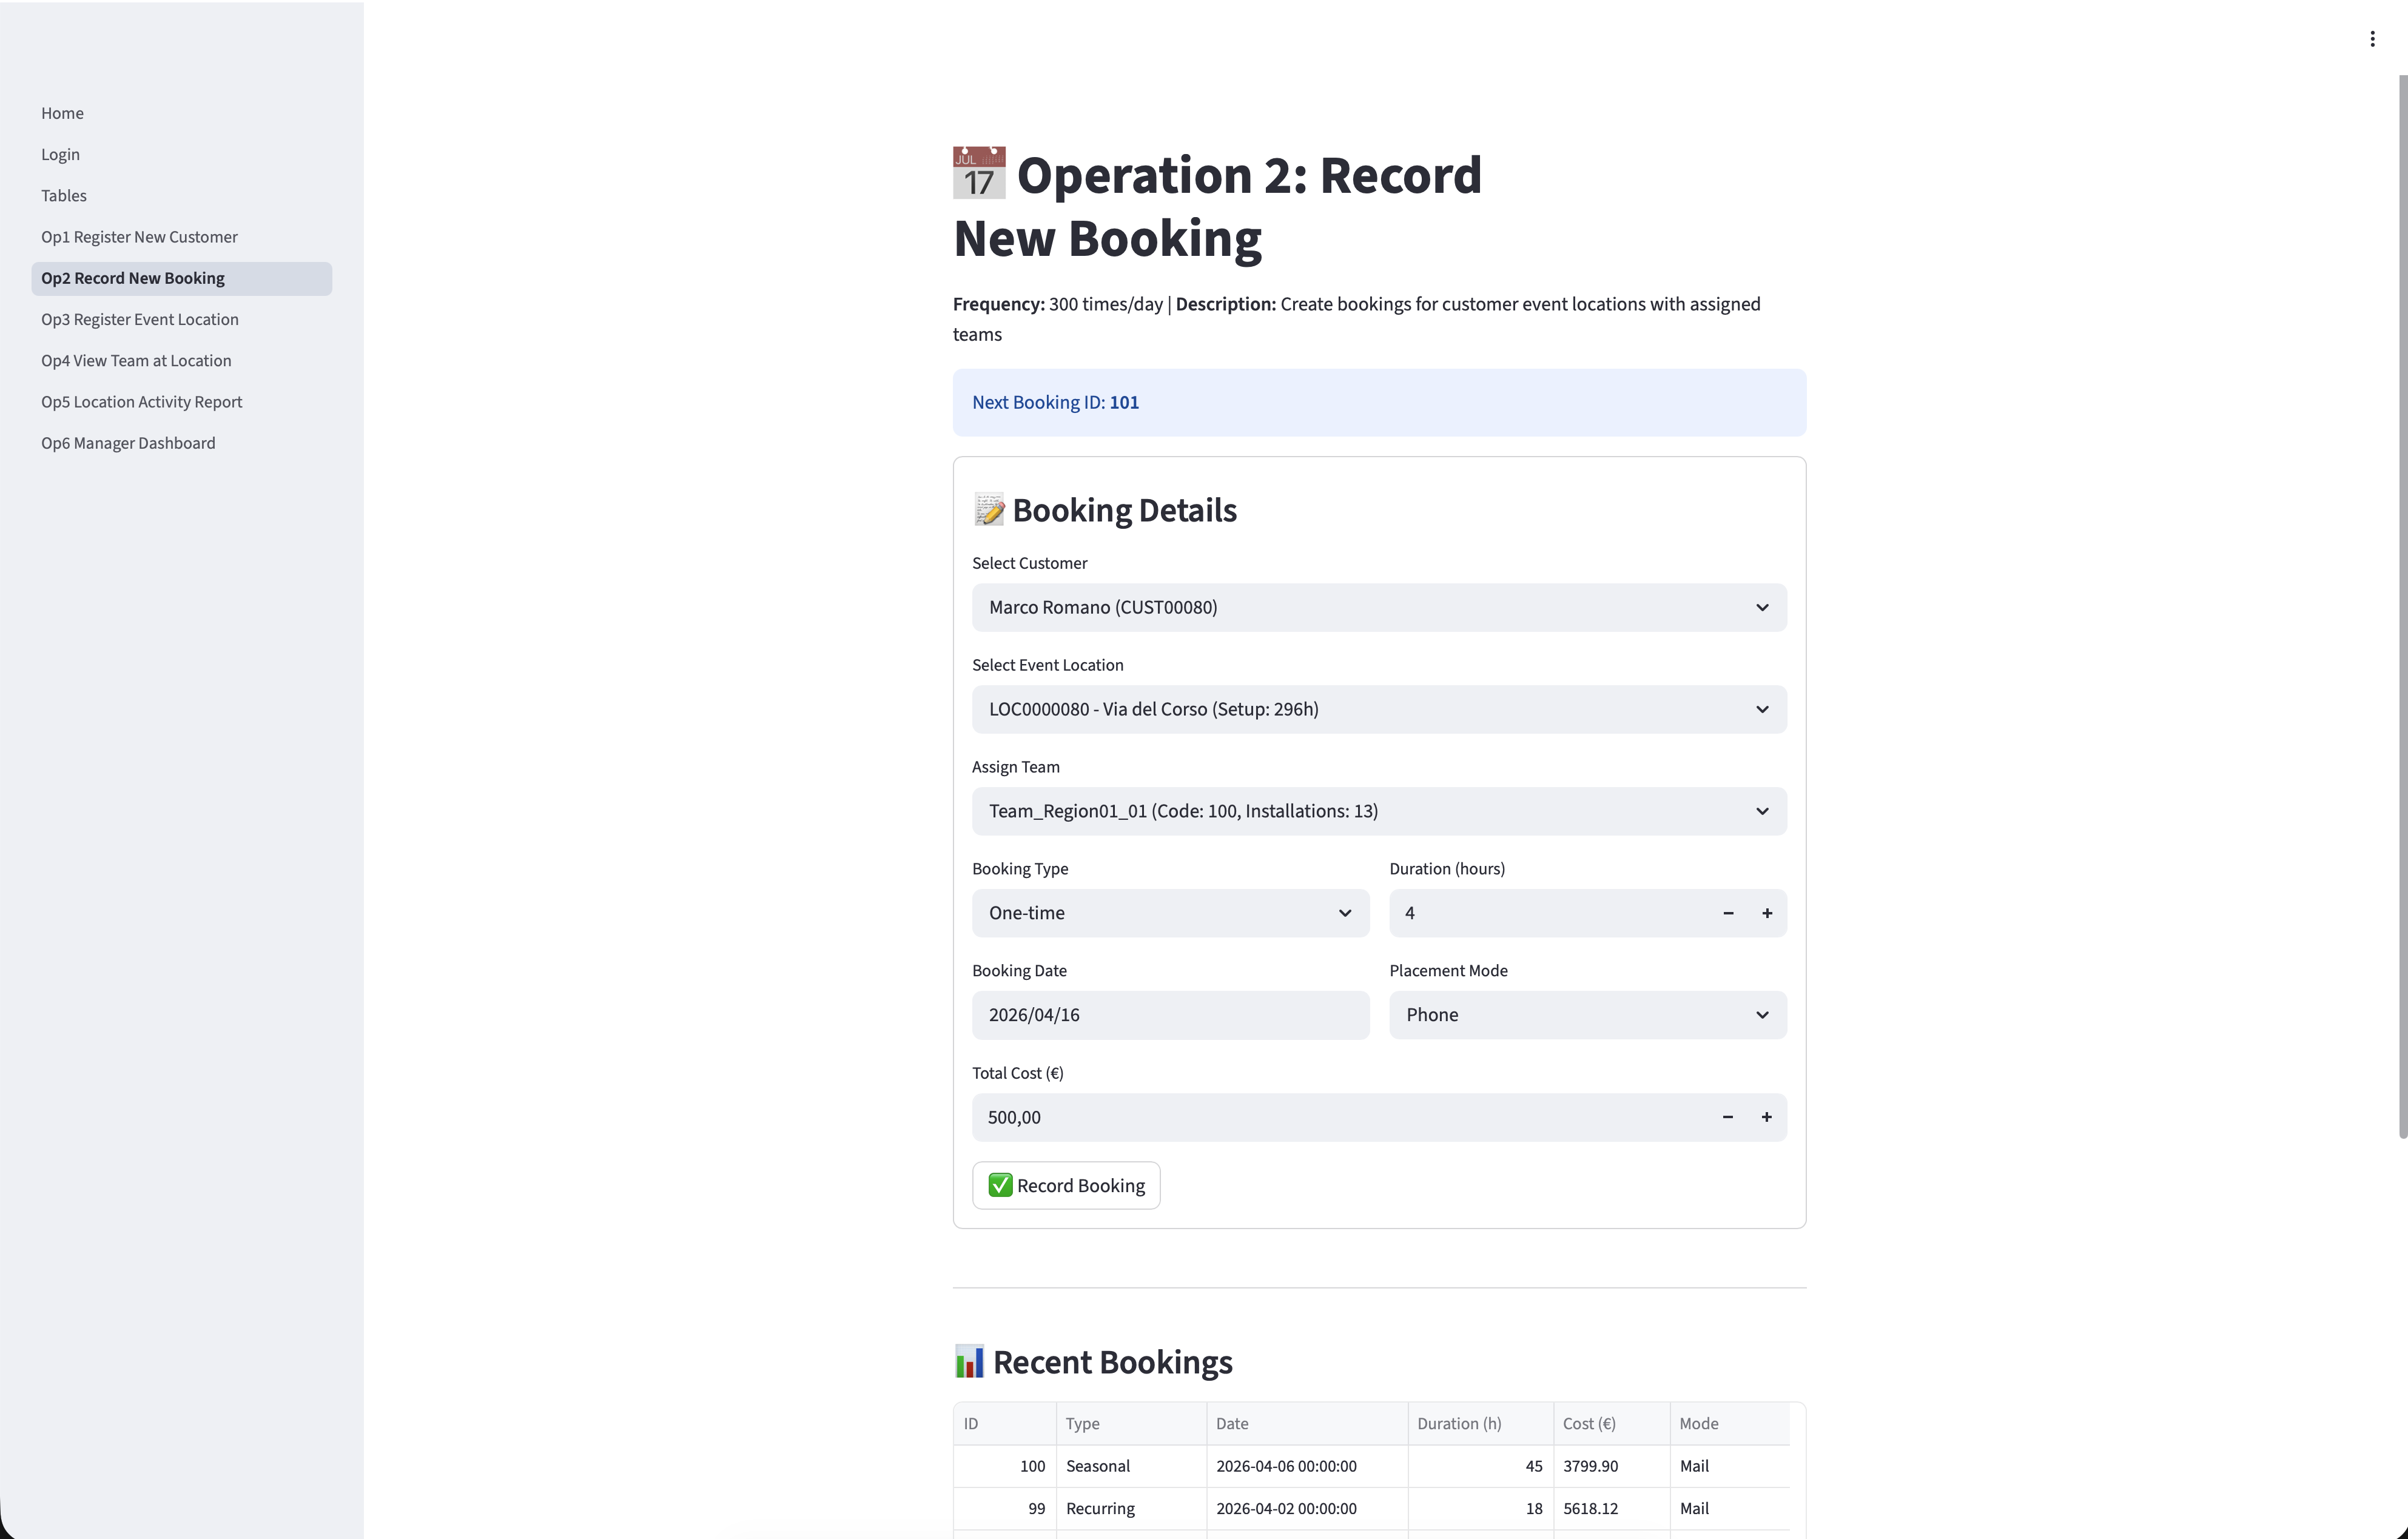
\includegraphics[width=0.72\textwidth]{images/streamlit_op2_record_booking.png}
    }{%
        \fbox{\parbox{0.8\textwidth}{\centering Insert screenshot: Operation 2 - Record New Booking}}
    }
    \caption{Interface for booking placement and assignment.}
\end{figure}

\subsubsection{Operation 3: Register New Event Location}
This operation is dedicated to the insertion of a new event location associated with an existing customer. The operator provides the full address and the technical attributes needed by the system, such as setup time estimate and supported equipment capacity.

\begin{figure}[H]
    \centering
    \IfFileExists{images/streamlit_op3_register_location.png}{%
        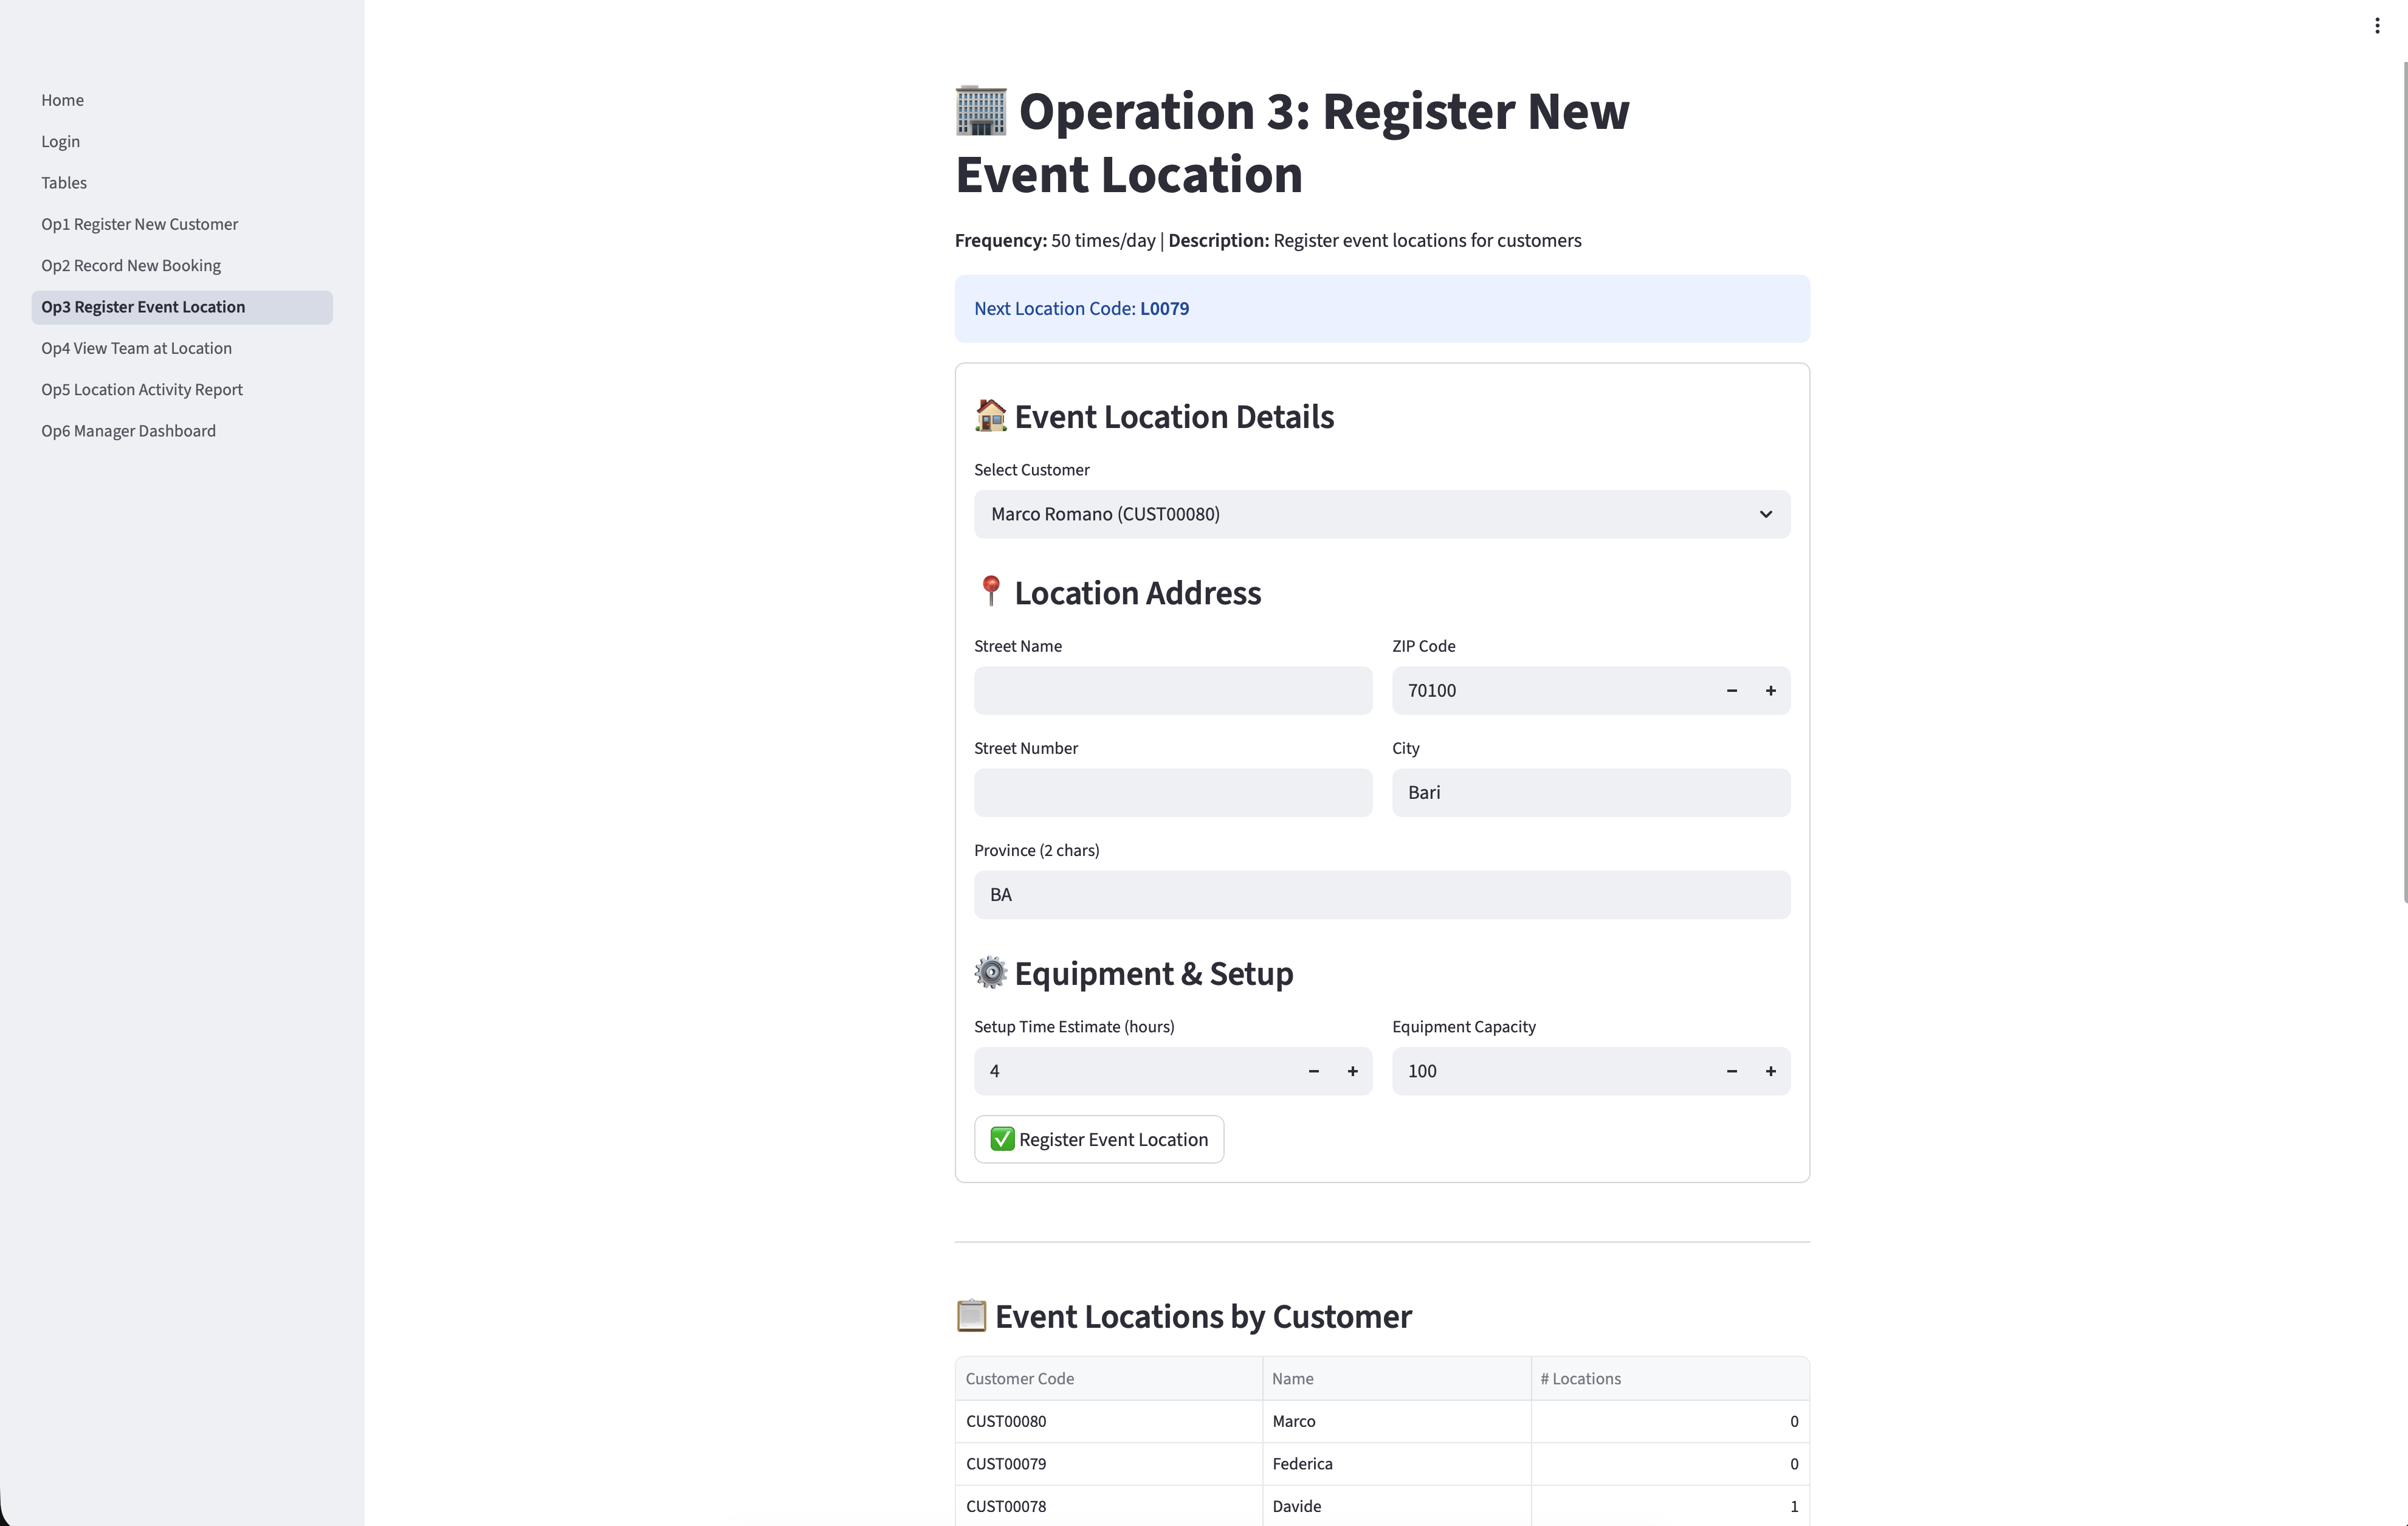
\includegraphics[width=0.72\textwidth]{images/streamlit_op3_register_location.png}
    }{%
        \fbox{\parbox{0.8\textwidth}{\centering Insert screenshot: Operation 3 - Register New Event Location}}
    }
    \caption{Interface for event-location registration.}
\end{figure}

\clearpage
\subsection{Team View}
This viewpoint focuses on the operational dimension of the \textbf{Setup Team}. It allows users to inspect which team handled a given event location, together with the associated office, booking details, and local performance indicators. In this way, the interface supports direct verification of field operations and helps reconstruct the operational context of each installation.

A second component of this viewpoint is the \textbf{Location Activity Report}, which ranks event locations according to the number of bookings handled. This page transforms operational records into a compact reporting tool, making it easier to identify the most active locations, compare demand across sites, and export the results for further analysis.

\begin{figure}[H]
    \centering
    \IfFileExists{images/streamlit_team_view_overview.png}{%
        \includegraphics[width=0.92\textwidth]{images/streamlit_team_view_overview.png}
    }{%
        \fbox{\parbox{0.85\textwidth}{\centering Insert screenshot: Team View Overview}}
    }
    \caption{Team-view overview page used to inspect teams, members, and related operational tables.}
\end{figure}

\subsubsection{Operation 4: View Team at Event Location}
This interface reconstructs the operational context of a selected event location. It shows the bookings linked to that site, the responsible office, the assigned setup team, and a compact summary of the local activity indicators useful for inspection.

\begin{figure}[H]
    \centering
    \IfFileExists{images/streamlit_op4_view_team_location.png}{%
        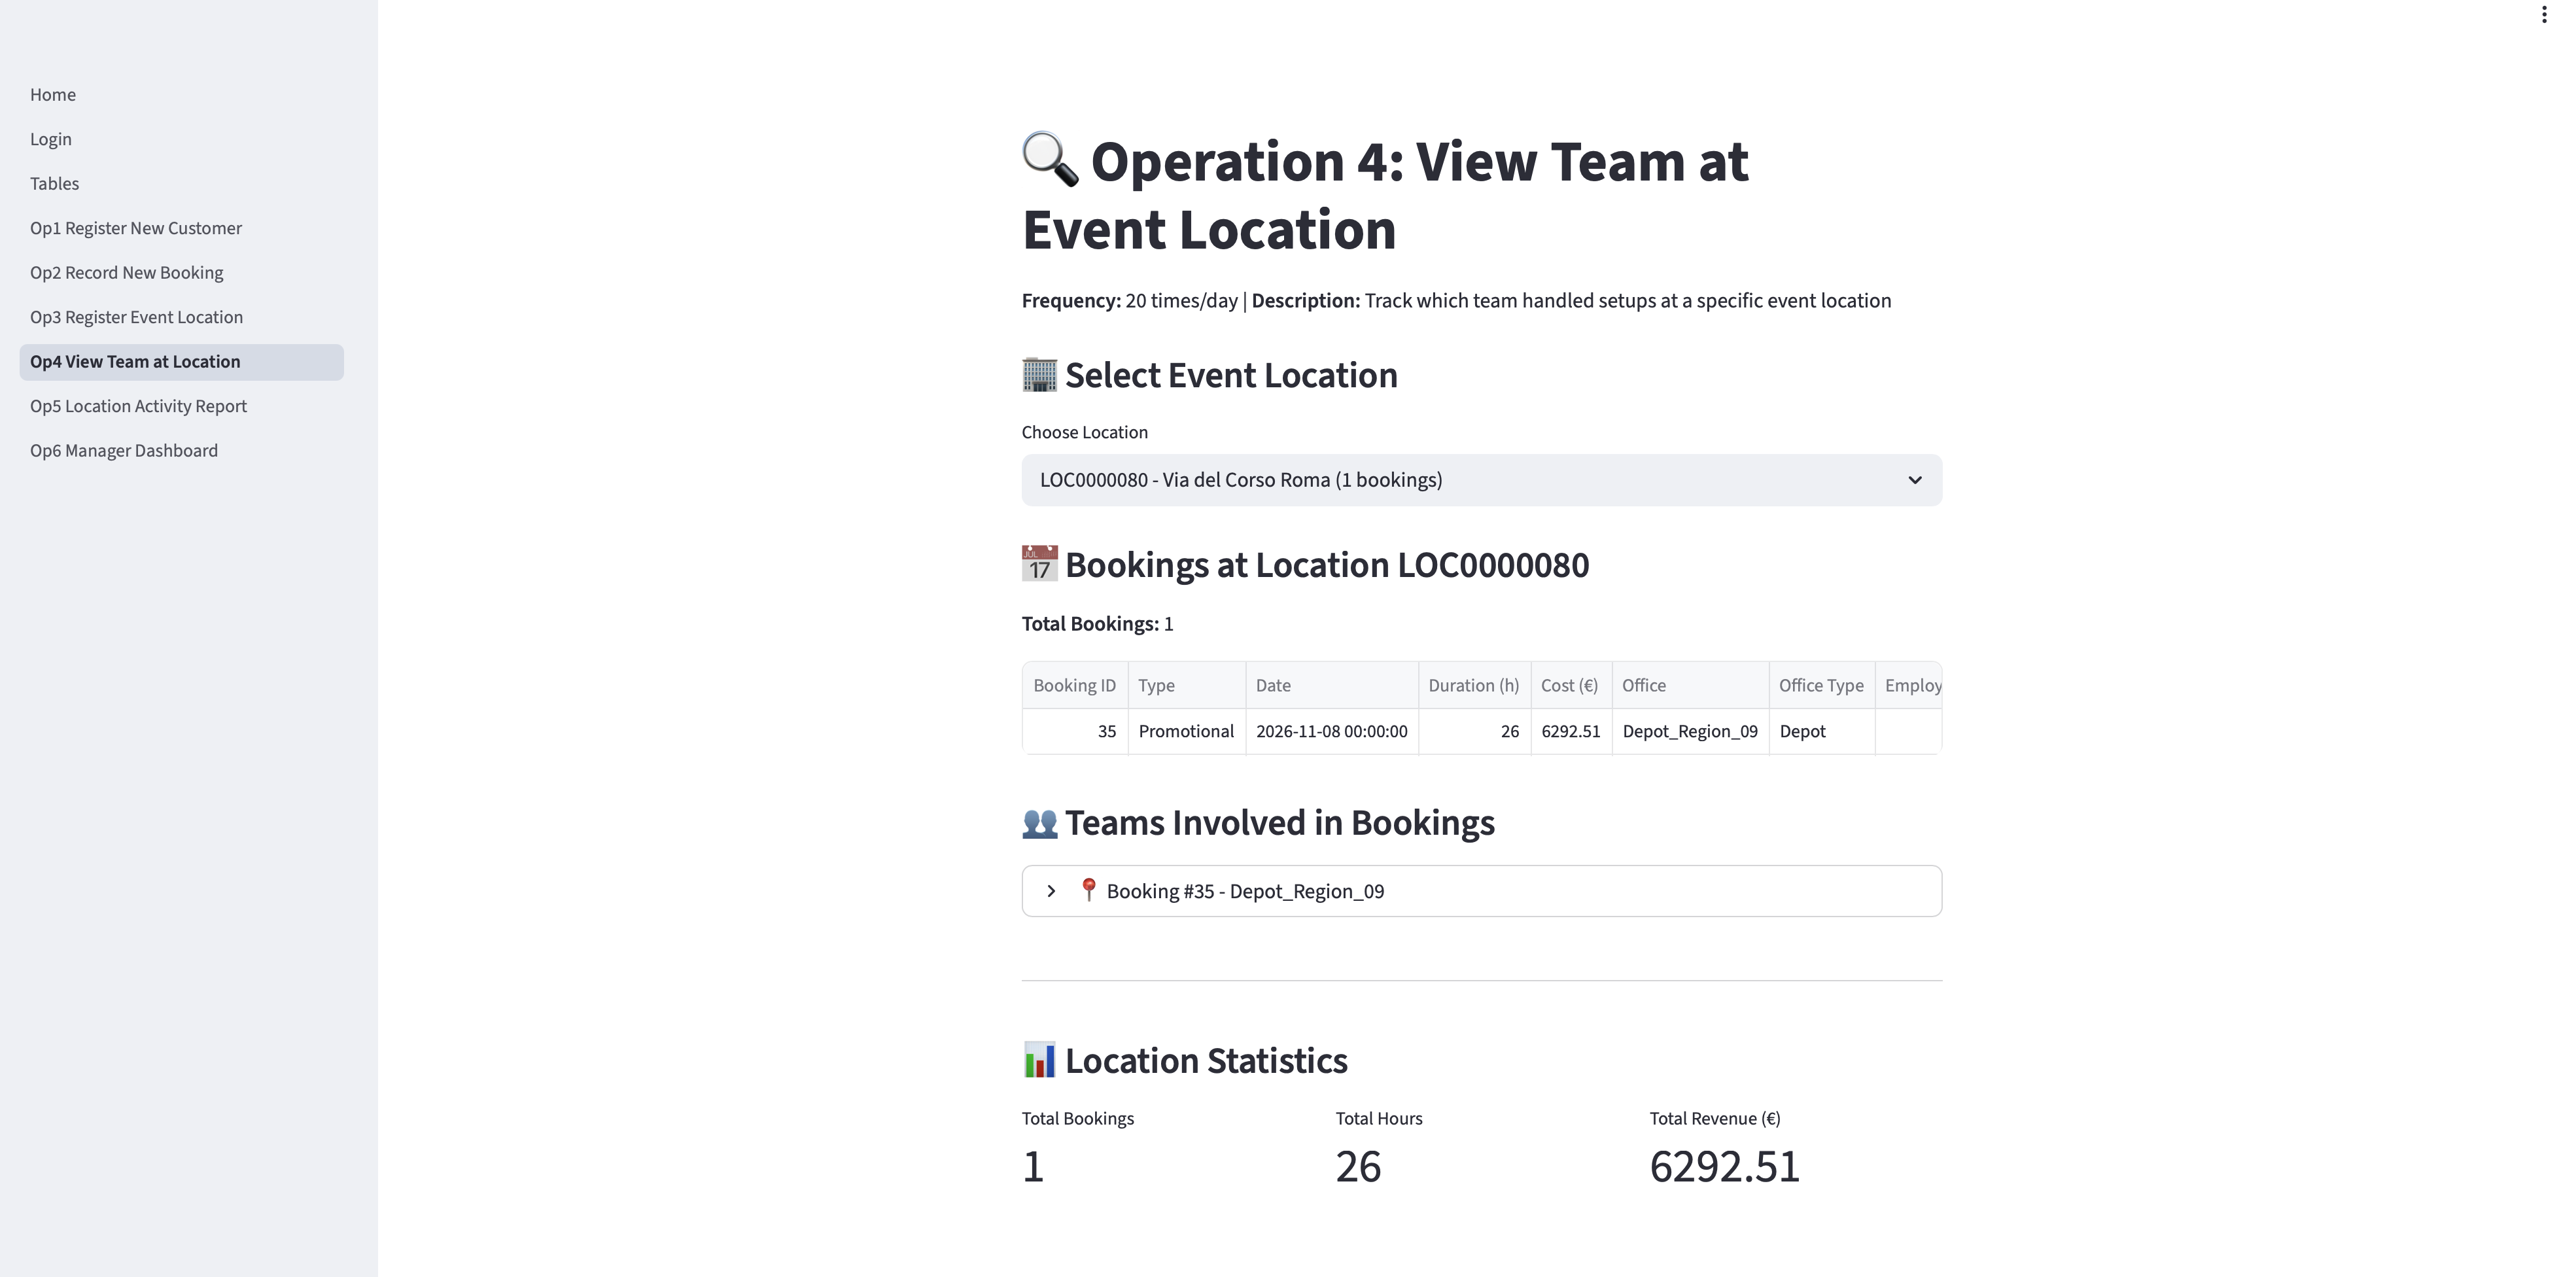
\includegraphics[width=0.72\textwidth]{images/streamlit_op4_view_team_location.png}
    }{%
        \fbox{\parbox{0.8\textwidth}{\centering Insert screenshot: Operation 4 - View Team at Event Location}}
    }
    \caption{Operational view for team inspection at a selected location.}
\end{figure}

\subsubsection{Operation 5: Location Activity Report}
This reporting page ranks event locations by the number of recorded bookings and summarizes the corresponding workload. The resulting table supports comparison across sites and can be exported for managerial or operational review.

\begin{figure}[H]
    \centering
    \IfFileExists{images/streamlit_op5_location_activity.png}{%
        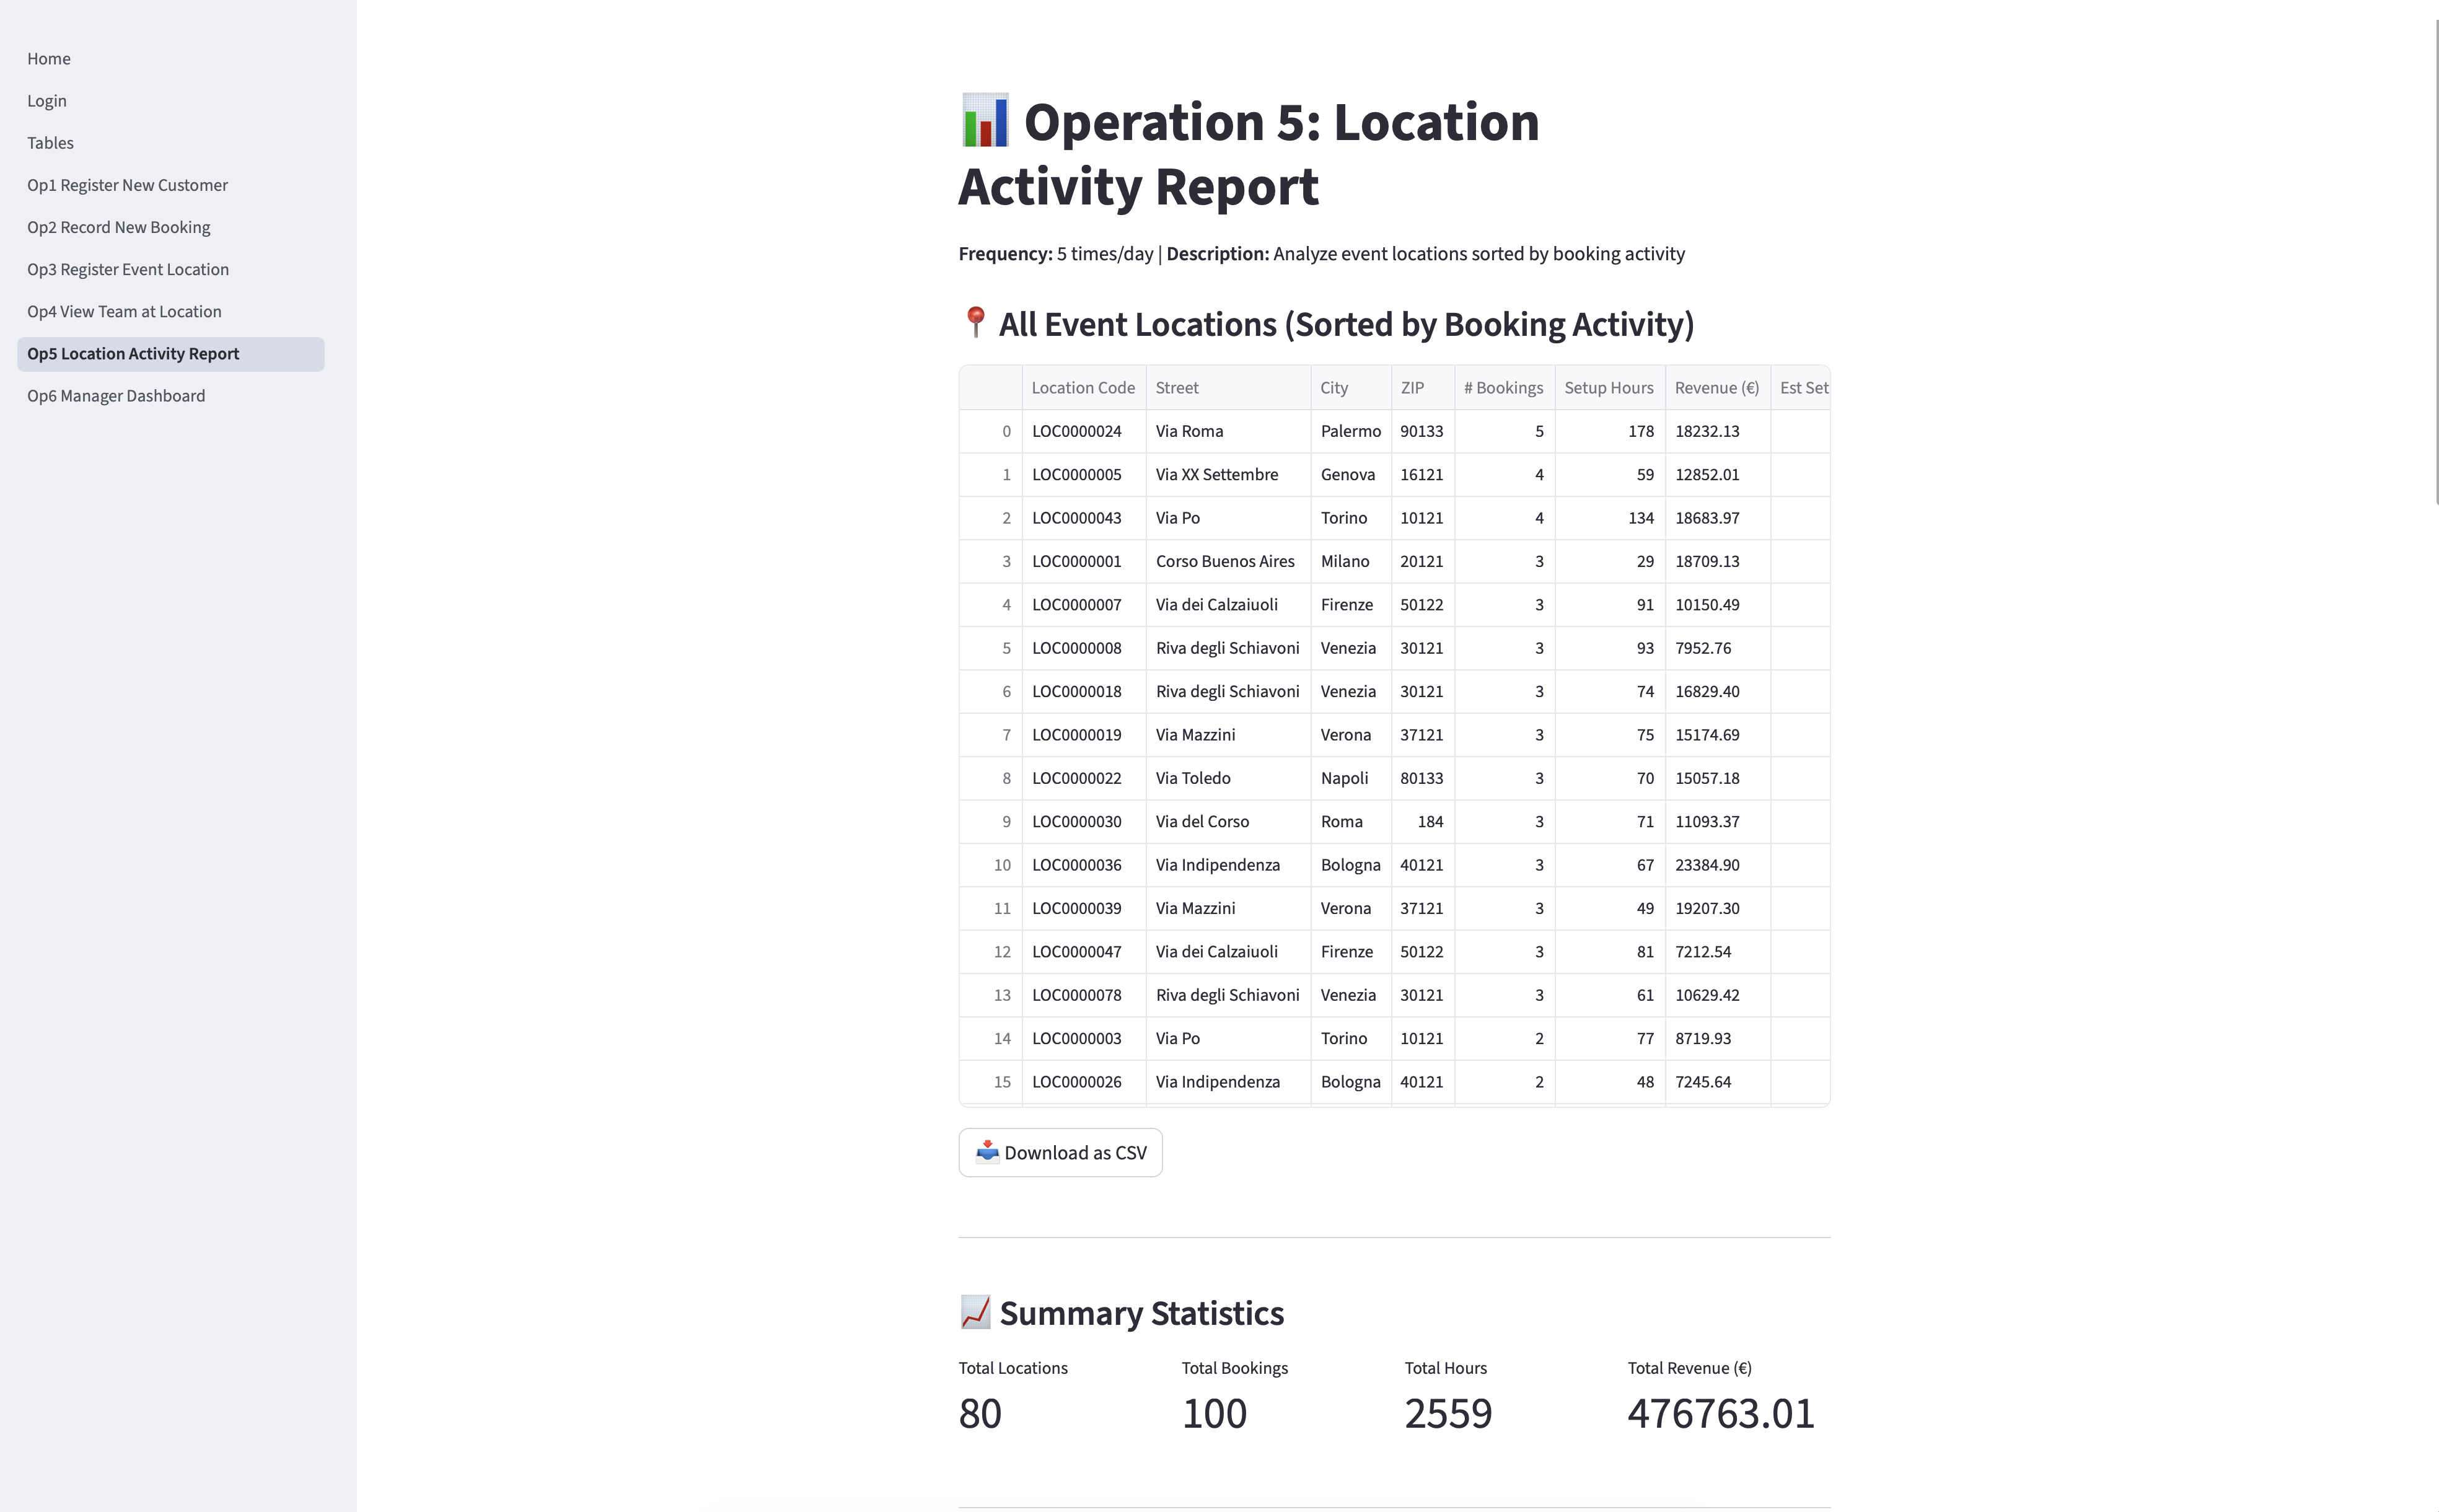
\includegraphics[width=0.72\textwidth]{images/streamlit_op5_location_activity.png}
    }{%
        \fbox{\parbox{0.8\textwidth}{\centering Insert screenshot: Operation 5 - Location Activity Report}}
    }
    \caption{Operational view for location activity analysis and ranking.}
\end{figure}

\clearpage
\subsection{Manager View}
The final managerial page provides a compact analytical cockpit built on top of the operational database. A performance area displays teams ordered by their score and installation volume, making comparative evaluation immediate. At the top of the dashboard, several global indicators are shown, including:

\begin{itemize}
    \item the total number of bookings tracked by the system;
    \item the total operational revenue generated;
    \item the average booking duration across the dataset;
    \item the number of active offices involved in the filtered result set.
\end{itemize}

The dashboard also includes historical demand charts, province-based distributions, booking-modality statistics, and office-level summary tables. Altogether, this view supports a broader interpretation of organizational performance and helps identify the most active teams, the most relevant operational areas, and the main historical demand trends.

\subsubsection{Operation 6: Manager Dashboard}
This page offers a consolidated analytical dashboard for supervisors and decision makers. It combines global KPIs, temporal trends, provincial distributions, and team-level comparisons in a single interface designed to support fast performance assessment.

\begin{figure}[H]
    \centering
    \IfFileExists{images/streamlit_op6_manager_dashboard.png}{%
        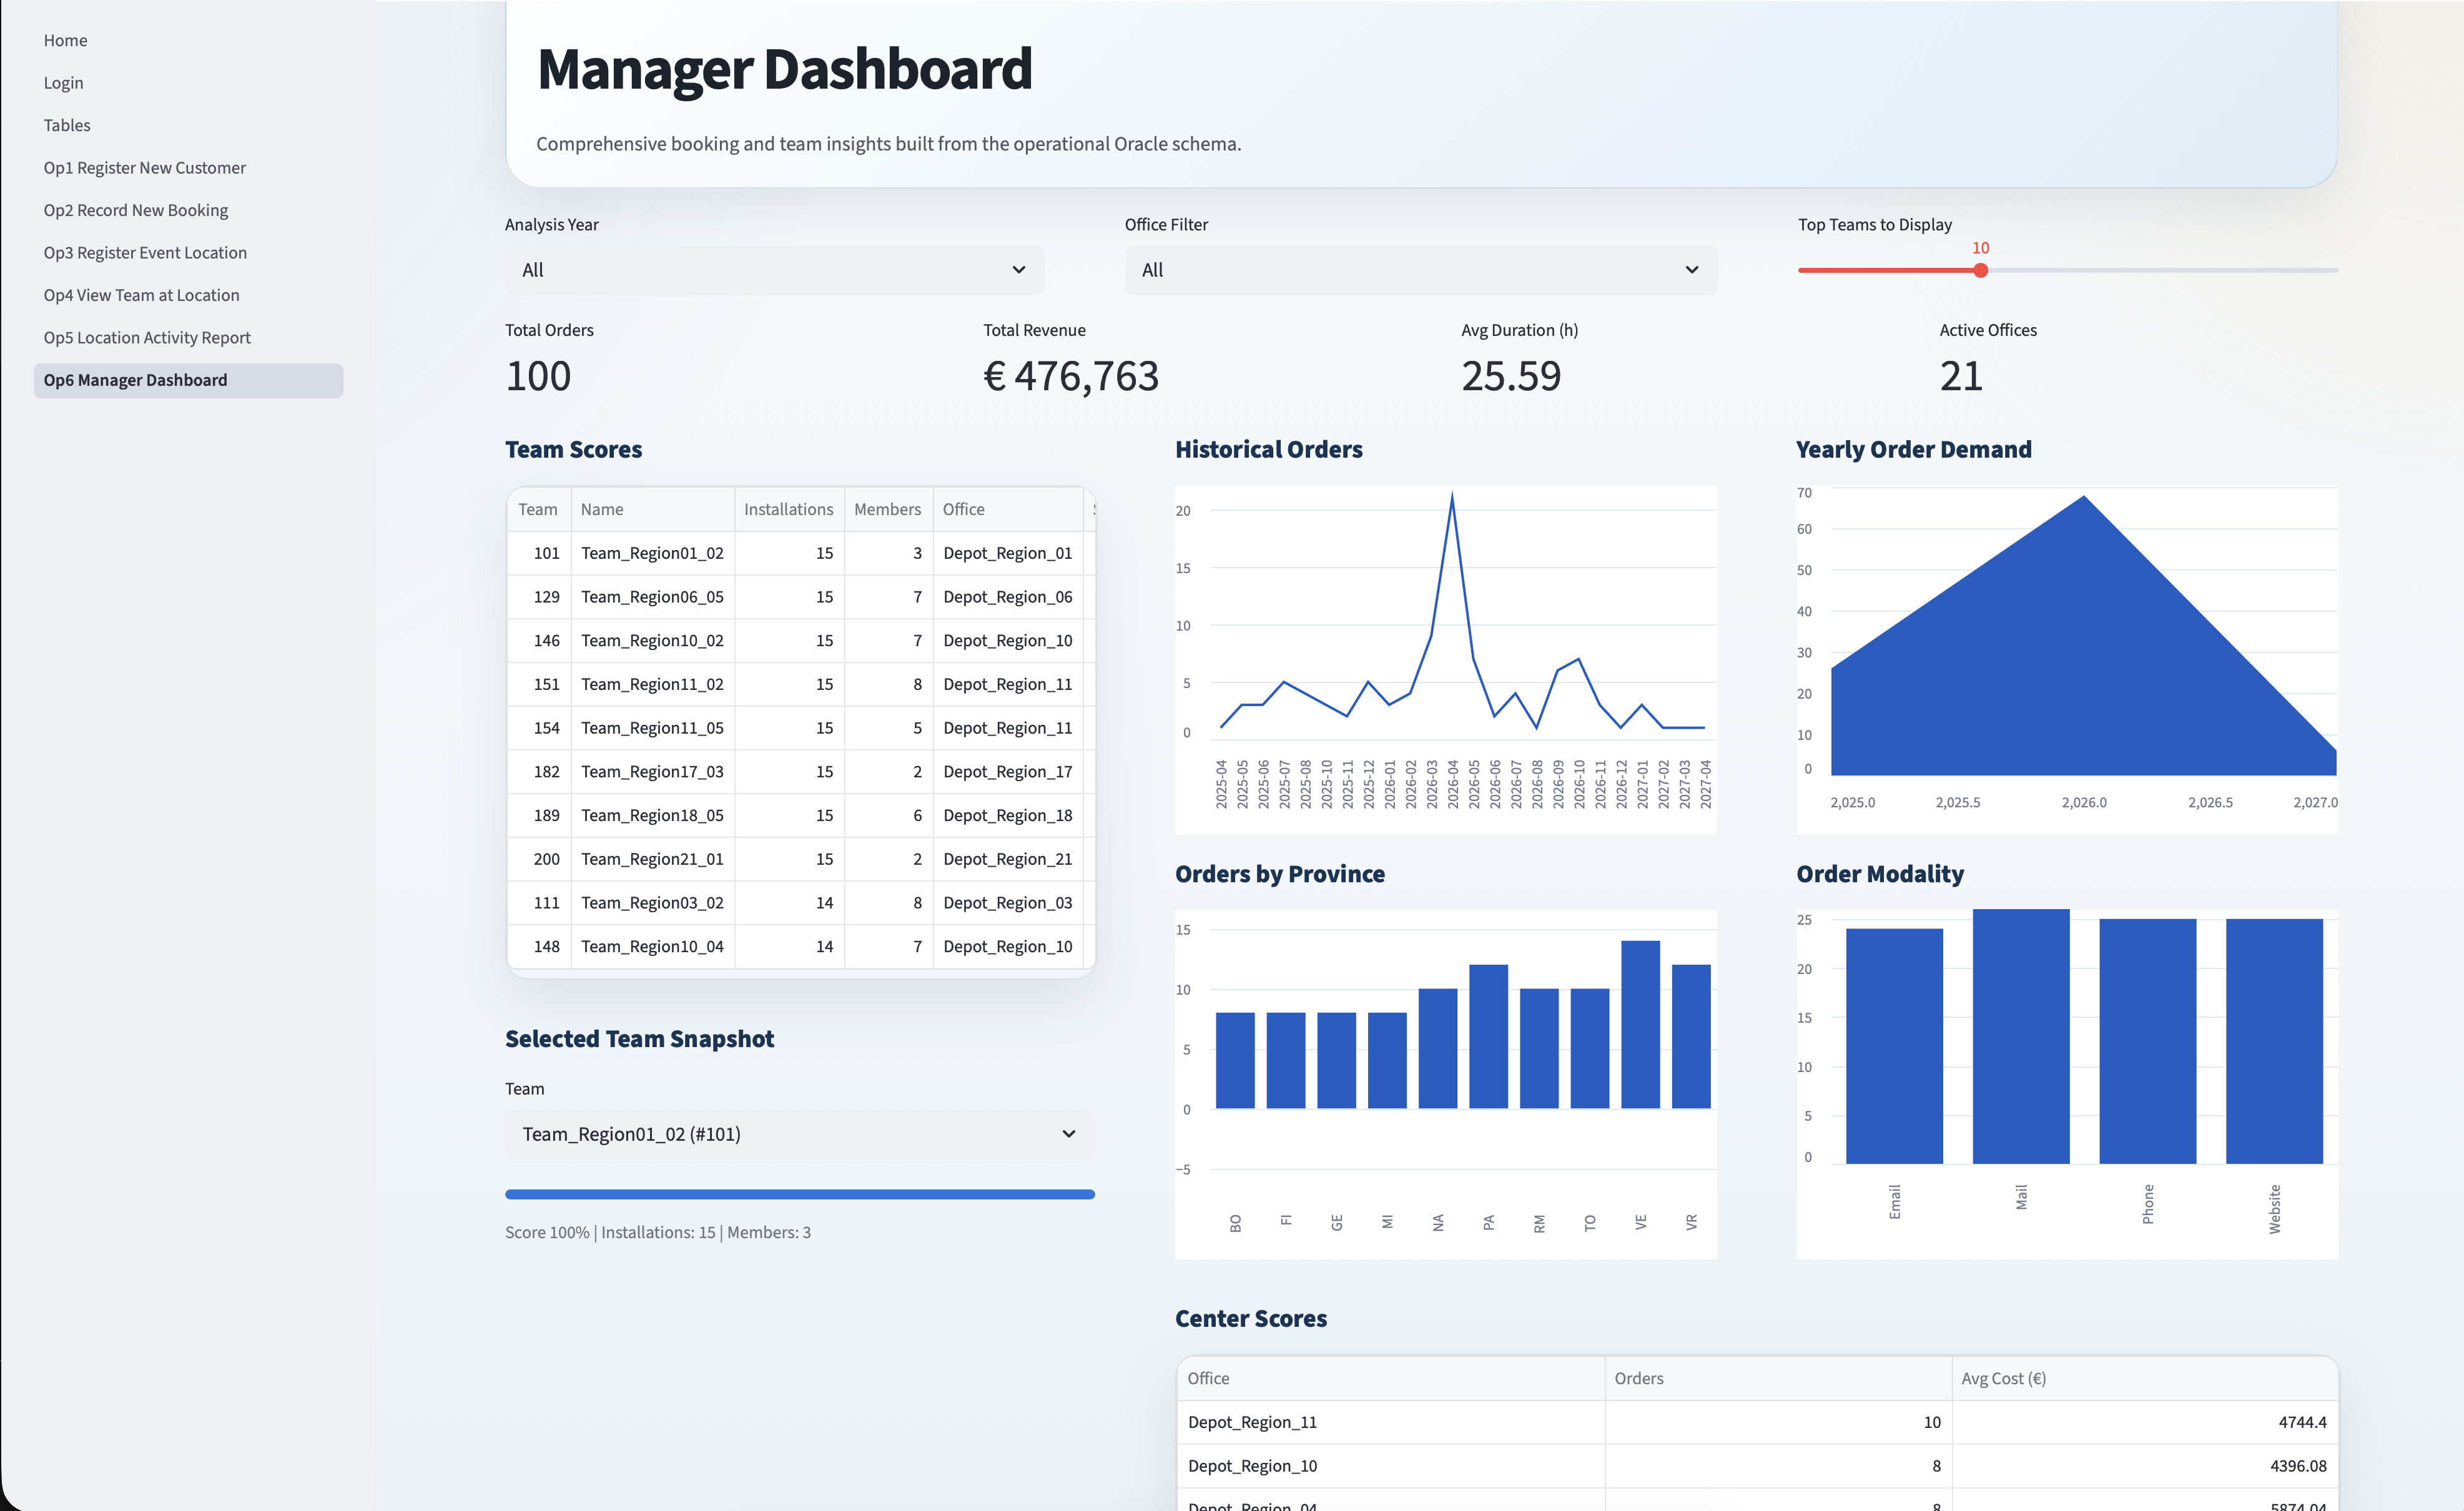
\includegraphics[width=0.78\textwidth]{images/streamlit_op6_manager_dashboard.png}
    }{%
        \fbox{\parbox{0.8\textwidth}{\centering Insert screenshot: Operation 6 - Manager Dashboard}}
    }
    \caption{Managerial dashboard with KPI indicators and historical trends.}
\end{figure}

\end{document}